\documentclass[11pt]{article}
\usepackage{amsmath,amssymb}
\usepackage{booktabs}
\usepackage{graphicx}
\usepackage{longtable}
\usepackage{hyperref}
\hypersetup{colorlinks=true,linkcolor=blue,citecolor=blue,urlcolor=blue}
\usepackage[margin=1in]{geometry}
\usepackage{natbib}
% Generated by rfsrealloc.pipeline; do not edit.

\newcommand{\valabsorbableDrawdown}{2.0}
\newcommand{\valadditionalAB}{250}
\newcommand{\valadditionalBBD}{180}
\newcommand{\valadditionalExactRF}{766.8}
\newcommand{\valadditionalRF}{770}
\newcommand{\valadditionalRFReportedBasis}{760}
\newcommand{\valbankBaseline}{4.37}
\newcommand{\valbankOutFirstAllTwoZeroTwoSeven}{3.37}
\newcommand{\valbankOutFirstEqual}{3.01}
\newcommand{\valbankOutFirstSetTwo}{3.37}
\newcommand{\valbankOutSecondAllTwoZeroTwoSeven}{1.56}
\newcommand{\valbankOutSecondEqual}{1.57}
\newcommand{\valbankOutSecondSetTwo}{2.33}
\newcommand{\valbankRia}{3.6}
\newcommand{\valbtFirstTargetYear}{2021}
\newcommand{\valbtLastTargetYear}{2027}
\newcommand{\valbtMaeAllSecond}{1,003}
\newcommand{\valbtMaeEqual}{969}
\newcommand{\valbtNTargetYears}{7}
\newcommand{\valbtNYearsFullyUnknownEqual}{6}
\newcommand{\valbtUnknownAllSecondFirst}{160}
\newcommand{\valbtUnknownAllSecondSecond}{1,760}
\newcommand{\valbtUnknownEqualFirst}{960}
\newcommand{\valbtUnknownEqualSecond}{880}
\newcommand{\valbtUnknownShareAllFirst}{1.0}
\newcommand{\valbtUnknownShareAllSecond}{0.876}
\newcommand{\valbtUnknownShareAllSecondFirst}{0.139}
\newcommand{\valbtUnknownShareAllSecondSecond}{1.0}
\newcommand{\valbtUnknownShareEqual}{0.932}
\newcommand{\valbtUnknownShareEqualFirst}{0.66}
\newcommand{\valbtUnknownShareEqualSecond}{1.0}
\newcommand{\valcapBindsAnywhere}{no}
\newcommand{\valcapFirstAllTwoZeroTwoSeven}{5.36}
\newcommand{\valcapFirstEqual}{5.44}
\newcommand{\valcapFirstSetTwo}{5.36}
\newcommand{\valcapSecondAllTwoZeroTwoSeven}{5.56}
\newcommand{\valcapSecondEqual}{5.48}
\newcommand{\valcapSecondSetTwo}{5.4}
\newcommand{\valcarryoverUsedFirstAllTwoZeroTwoSeven}{4.37}
\newcommand{\valcarryoverUsedFirstEqual}{4.37}
\newcommand{\valcarryoverUsedFirstSetTwo}{4.37}
\newcommand{\valcarryoverUsedSecondAllTwoZeroTwoSeven}{3.37}
\newcommand{\valcarryoverUsedSecondEqual}{3.01}
\newcommand{\valcarryoverUsedSecondSetTwo}{3.37}
\newcommand{\valconfigHash}{f45a4a00633f4fe8}
\newcommand{\valconfigName}{paper}
\newcommand{\valcostRelFirstAllTwoZeroTwoSeven}{0.0}
\newcommand{\valcostRelFirstEqual}{0.37}
\newcommand{\valcostRelSecondAllTwoZeroTwoSeven}{0.79}
\newcommand{\valcostRelSecondEqual}{0.4}
\newcommand{\valcrossCheckBbdReduction}{0.31}
\newcommand{\valcrossCheckExtraExemptFuel}{5.83}
\newcommand{\valcrossCheckRfReduction}{0.9}
\newcommand{\valdStdPerOneZeroZeroMRinsFirst}{0.0578}
\newcommand{\valdStdPerOneZeroZeroMRinsSecond}{0.0584}
\newcommand{\valdeadlineDaysScenarioHypotheticalEarlyTwoZeroTwoSeven}{58}
\newcommand{\valdeadlineDaysScenarioHypotheticalLateTwoZeroTwoSeven}{61}
\newcommand{\valdeadlineDaysScenarioHypotheticalMidTwoZeroTwoSeven}{92}
\newcommand{\valdeadlineNotFinalized}{2027-12-01}
\newcommand{\valdeadlineScenarioHypotheticalEarlyTwoZeroTwoSeven}{2027-03-31}
\newcommand{\valdeadlineScenarioHypotheticalLateTwoZeroTwoSeven}{2027-12-01}
\newcommand{\valdeadlineScenarioHypotheticalMidTwoZeroTwoSeven}{2027-09-01}
\newcommand{\valdeficitFirstAllTwoZeroTwoSeven}{0.0}
\newcommand{\valdeficitFirstEqual}{0.0}
\newcommand{\valdeficitFirstSetTwo}{0.0}
\newcommand{\valdeficitSecondAllTwoZeroTwoSeven}{0.0}
\newcommand{\valdeficitSecondEqual}{0.0}
\newcommand{\valdeficitSecondSetTwo}{0.0}
\newcommand{\valdenominatorFirst}{173.02}
\newcommand{\valdenominatorSecond}{171.24}
\newcommand{\valdrawdownExcessOverAbsorbableAllSecond}{0.81}
\newcommand{\valdrawdownExcessOverAbsorbableEqual}{0.8}
\newcommand{\valdrawdownTwoYearsAllSecond}{2.81}
\newcommand{\valdrawdownTwoYearsEqual}{2.8}
\newcommand{\valdrawdownTwoYearsSetTwo}{2.04}
\newcommand{\valervoMismatchDescription}{2024 AB: computed 290, published 300}
\newcommand{\valervoMismatchMinVolumeBgal}{7.7836}
\newcommand{\valfuelErrorMaxPct}{6.0}
\newcommand{\valfuelErrorMeanPct}{2.19}
\newcommand{\valfuelErrorMinPct}{-3.71}
\newcommand{\valfuelErrorSdPct}{2.79}
\newcommand{\valimpliedDenominatorHiFirst}{173.024}
\newcommand{\valimpliedDenominatorHiSecond}{171.244}
\newcommand{\valimpliedDenominatorLoFirst}{173.019}
\newcommand{\valimpliedDenominatorLoSecond}{171.203}
\newcommand{\vallagTwoZeroTwoFourMedianYears}{0.64}
\newcommand{\vallagTwoZeroTwoFiveMedianYears}{0.66}
\newcommand{\vallagMaxYears}{3.85}
\newcommand{\vallagMedianYears}{1.64}
\newcommand{\vallagMinYears}{0.64}
\newcommand{\vallagYearsFirst}{2021}
\newcommand{\vallagYearsLast}{2025}
\newcommand{\vallaterShareTwoZeroTwoFourPct}{16.2}
\newcommand{\valmaxAbsResidualPoints}{0.0049}
\newcommand{\valmcDraws}{100,000}
\newcommand{\valmcseHeadlineRelative}{0.00224}
\newcommand{\valnCostChecked}{6}
\newcommand{\valnCostMatched}{6}
\newcommand{\valnDoubleEntryMismatches}{0}
\newcommand{\valnErvoChecked}{12}
\newcommand{\valnErvoMatched}{11}
\newcommand{\valnFrParsedValuesCompared}{156}
\newcommand{\valnFrParsedValuesMismatched}{0}
\newcommand{\valnFuelErrorsAll}{15}
\newcommand{\valnFuelErrorsProspective}{9}
\newcommand{\valnLagPetitions}{153}
\newcommand{\valnPendingTwoZeroTwoFive}{2}
\newcommand{\valnPendingTwoZeroTwoSix}{7}
\newcommand{\valnPendingTwoZeroTwoSeven}{4}
\newcommand{\valnProjYears}{10}
\newcommand{\valnProjYearsRealTime}{7}
\newcommand{\valnRevisionPairs}{7}
\newcommand{\valnSrervFloorCeilMatched}{6}
\newcommand{\valnSrervNearestMatched}{3}
\newcommand{\valnStandardsChangedByReportedBasis}{2}
\newcommand{\valnStandardsChecked}{32}
\newcommand{\valnStandardsMatched}{32}
\newcommand{\valnTableIVOneChecked}{12}
\newcommand{\valnTableIVOneMatched}{12}
\newcommand{\valnewRinsFirstAllTwoZeroTwoSeven}{22.45}
\newcommand{\valnewRinsFirstEqual}{22.81}
\newcommand{\valnewRinsFirstEqualMinusAllSecond}{0.36}
\newcommand{\valnewRinsFirstSetTwo}{22.45}
\newcommand{\valnewRinsSecondAbsDiffEqualAllSecond}{0.01}
\newcommand{\valnewRinsSecondAllTwoZeroTwoSeven}{24.42}
\newcommand{\valnewRinsSecondEqual}{24.41}
\newcommand{\valnewRinsSecondSetTwo}{23.65}
\newcommand{\valprojMaeHindsight}{476}
\newcommand{\valprojMaeHindsightPct}{42.1}
\newcommand{\valprojMaeRealTime}{1,090}
\newcommand{\valprojMaxAbsHindsight}{1,390}
\newcommand{\valrealizedMinusIntendedMeanFirstAllSecond}{0.458}
\newcommand{\valrealizedMinusIntendedMeanFirstEqual}{0.42}
\newcommand{\valrealizedMinusIntendedMeanSecondAllSecond}{0.518}
\newcommand{\valrealizedMinusIntendedMeanSecondEqual}{0.555}
\newcommand{\valrealizedMinusIntendedQZeroFiveFirstAllSecond}{-1.062}
\newcommand{\valrealizedMinusIntendedQZeroFiveFirstEqual}{-1.12}
\newcommand{\valrealizedMinusIntendedQZeroFiveSecondAllSecond}{-1.157}
\newcommand{\valrealizedMinusIntendedQZeroFiveSecondEqual}{-1.095}
\newcommand{\valrealizedMinusIntendedQNineFiveFirstAllSecond}{1.391}
\newcommand{\valrealizedMinusIntendedQNineFiveFirstEqual}{1.373}
\newcommand{\valrealizedMinusIntendedQNineFiveSecondAllSecond}{1.699}
\newcommand{\valrealizedMinusIntendedQNineFiveSecondEqual}{1.706}
\newcommand{\valrealizedMinusIntendedSdFirstAllSecond}{0.7}
\newcommand{\valrealizedMinusIntendedSdFirstEqual}{0.712}
\newcommand{\valrealizedMinusIntendedSdSecondAllSecond}{0.803}
\newcommand{\valrealizedMinusIntendedSdSecondEqual}{0.785}
\newcommand{\valreportedTwoZeroTwoFiveExemptedRvo}{1,750}
\newcommand{\valreportedTwoZeroTwoFiveExemptedVolume}{13,326}
\newcommand{\valreportedTwoZeroTwoFiveRatio}{0.9943}
\newcommand{\valreportedBasisMaxChangePoints}{0.01}
\newcommand{\valreportedBasisStdSecondAllSecond}{16.22}
\newcommand{\valreportedBasisStdSecondEqual}{16.00}
\newcommand{\valretroAllSecondScenarioHypotheticalEarlyTwoZeroTwoSeven}{0.085}
\newcommand{\valretroAllSecondScenarioHypotheticalLateTwoZeroTwoSeven}{0.748}
\newcommand{\valretroAllSecondScenarioHypotheticalMidTwoZeroTwoSeven}{0.414}
\newcommand{\valretroEqualScenarioHypotheticalEarlyTwoZeroTwoSeven}{0.542}
\newcommand{\valretroEqualScenarioHypotheticalLateTwoZeroTwoSeven}{0.874}
\newcommand{\valretroEqualScenarioHypotheticalMidTwoZeroTwoSeven}{0.707}
\newcommand{\valrevisionMeanAbsBRinsSecondAllSecond}{0.12}
\newcommand{\valrevisionMeanAbsFirstAllSecond}{0.0}
\newcommand{\valrevisionMeanAbsFirstEqual}{0.0344}
\newcommand{\valrevisionMeanAbsSecondAllSecond}{0.0695}
\newcommand{\valrevisionMeanAbsSecondEqual}{0.0347}
\newcommand{\valrevisionRatioMax}{1.014}
\newcommand{\valrevisionRatioMean}{0.95}
\newcommand{\valrevisionRatioMin}{0.828}
\newcommand{\valrevisionRatioSd}{0.067}
\newcommand{\valrvoFirstAllTwoZeroTwoSeven}{26.82}
\newcommand{\valrvoFirstEqual}{27.18}
\newcommand{\valrvoFirstSetTwo}{26.82}
\newcommand{\valrvoSecondAllTwoZeroTwoSeven}{27.79}
\newcommand{\valrvoSecondEqual}{27.42}
\newcommand{\valrvoSecondSetTwo}{27.02}
\newcommand{\valsensIndependentFuelRealizedMinusIntendedSdSecondAllSecond}{0.802}
\newcommand{\valsensIndependentFuelRealizedMinusIntendedSdSecondAllSecondIncreasePct}{-0.1}
\newcommand{\valsensIndependentFuelRealizedMinusIntendedSdSecondEqual}{0.784}
\newcommand{\valsensIndependentFuelRealizedMinusIntendedSdSecondEqualIncreasePct}{-0.1}
\newcommand{\valsensIndependentFuelRevisionMeanAbsFirstEqual}{0.0344}
\newcommand{\valsensIndependentFuelRevisionMeanAbsFirstEqualIncreasePct}{0.0}
\newcommand{\valsensIndependentFuelRevisionMeanAbsSecondAllSecond}{0.0695}
\newcommand{\valsensIndependentFuelRevisionMeanAbsSecondAllSecondIncreasePct}{0.0}
\newcommand{\valsensIndependentFuelStdSdFirstEqual}{0.037}
\newcommand{\valsensIndependentFuelStdSdFirstEqualIncreasePct}{0.0}
\newcommand{\valsensIndependentFuelStdSdSecondAllSecond}{0.0748}
\newcommand{\valsensIndependentFuelStdSdSecondAllSecondIncreasePct}{0.0}
\newcommand{\valsensUniformRealizedMinusIntendedSdSecondAllSecond}{0.82}
\newcommand{\valsensUniformRealizedMinusIntendedSdSecondAllSecondIncreasePct}{2.1}
\newcommand{\valsensUniformRealizedMinusIntendedSdSecondEqual}{0.789}
\newcommand{\valsensUniformRealizedMinusIntendedSdSecondEqualIncreasePct}{0.5}
\newcommand{\valsensUniformRevisionMeanAbsFirstEqual}{0.0509}
\newcommand{\valsensUniformRevisionMeanAbsFirstEqualIncreasePct}{48.0}
\newcommand{\valsensUniformRevisionMeanAbsSecondAllSecond}{0.1029}
\newcommand{\valsensUniformRevisionMeanAbsSecondAllSecondIncreasePct}{48.1}
\newcommand{\valsensUniformStdSdFirstEqual}{0.0588}
\newcommand{\valsensUniformStdSdFirstEqualIncreasePct}{58.9}
\newcommand{\valsensUniformStdSdSecondAllSecond}{0.1188}
\newcommand{\valsensUniformStdSdSecondAllSecondIncreasePct}{58.8}
\newcommand{\valshareABMINUSBBD}{0.0883}
\newcommand{\valshareBBD}{0.2399}
\newcommand{\valshareCB}{0.0541}
\newcommand{\valshareCONV}{0.6717}
\newcommand{\valshareOA}{0.0343}
\newcommand{\valsobolFuelRealizedFirstAllSecond}{1.0}
\newcommand{\valsobolFuelRealizedFirstEqual}{0.992}
\newcommand{\valsobolFuelRealizedSecondAllSecond}{0.979}
\newcommand{\valsobolFuelRealizedSecondEqual}{0.994}
\newcommand{\valsobolFuelStdFirstAllSecond}{0.0}
\newcommand{\valsobolFuelStdFirstEqual}{0.0}
\newcommand{\valsobolFuelStdSecondAllSecond}{0.0}
\newcommand{\valsobolFuelStdSecondEqual}{0.0}
\newcommand{\valsobolRevisionRealizedFirstAllSecond}{0.0}
\newcommand{\valsobolRevisionRealizedFirstEqual}{0.008}
\newcommand{\valsobolRevisionRealizedSecondAllSecond}{0.021}
\newcommand{\valsobolRevisionRealizedSecondEqual}{0.006}
\newcommand{\valsobolRevisionStdFirstAllSecond}{0.0}
\newcommand{\valsobolRevisionStdFirstEqual}{1.0}
\newcommand{\valsobolRevisionStdSecondAllSecond}{1.0}
\newcommand{\valsobolRevisionStdSecondEqual}{1.0}
\newcommand{\valstdMeanFirstAllSecond}{15.495}
\newcommand{\valstdMeanFirstEqual}{15.692}
\newcommand{\valstdMeanSecondAllSecond}{16.177}
\newcommand{\valstdMeanSecondEqual}{15.978}
\newcommand{\valstdQZeroFiveFirstAllSecond}{15.495}
\newcommand{\valstdQZeroFiveFirstEqual}{15.624}
\newcommand{\valstdQZeroFiveSecondAllSecond}{16.039}
\newcommand{\valstdQZeroFiveSecondEqual}{15.909}
\newcommand{\valstdQNineFiveFirstAllSecond}{15.495}
\newcommand{\valstdQNineFiveFirstEqual}{15.745}
\newcommand{\valstdQNineFiveSecondAllSecond}{16.284}
\newcommand{\valstdQNineFiveSecondEqual}{16.032}
\newcommand{\valstdSdFirstAllSecond}{0.0}
\newcommand{\valstdSdFirstEqual}{0.037}
\newcommand{\valstdSdSecondAllSecond}{0.0748}
\newcommand{\valstdSdSecondEqual}{0.0374}
\newcommand{\valstepAllSecondBRinsSecond}{0.77}
\newcommand{\valstepEqualBRinsFirst}{0.38}
\newcommand{\valstepEqualBRinsSecond}{0.38}
\newcommand{\valstepFirstEqual}{0.223}
\newcommand{\valstepSecondAllSecond}{0.45}
\newcommand{\valstepSecondEqual}{0.225}

\graphicspath{{figures/}}
\title{Supporting Information for ``Reallocating exempted obligations under the Renewable Fuel Standard: exact reconstruction, uncertainty propagation and the predictability of alternative timing rules''}
\author{Avin Gupta}
\date{}
\begin{document}
\maketitle

\section{Code-to-equation map}

\begin{tabular}{p{0.42\textwidth}p{0.52\textwidth}}
\toprule
Equation or quantity & Implementation \\
\midrule
Percentage standard, 40 CFR 80.1405(c) & \texttt{rfsrealloc.standards.standards}, \texttt{obligated\_volume} (exact rationals) \\
Rounding to two decimals, half-up & \texttt{rfsrealloc.standards.round\_half\_up} \\
Implied denominator interval & \texttt{rfsrealloc.standards.implied\_denominator\_interval} \\
Exempted obligation $\mathrm{ERVO}_{X,y}$ & \texttt{rfsrealloc.reallocation.exempted\_rvo}, \texttt{ervo\_table} \\
Set 2 reallocation volumes (floor 2026, ceiling 2027) & \texttt{rfsrealloc.reallocation.set2\_srerv}, \texttt{round\_to} \\
Additional 2025 obligation $A_X$ & \texttt{rfsrealloc.reallocation.additional\_ervo} \\
Timing-rule family $w$ & \texttt{rfsrealloc.reallocation.allocate}; \texttt{uncertainty.TimingModel.standards} \\
Retroactivity $R(w,t)$ & \texttt{rfsrealloc.reallocation.retroactivity} \\
Revision ratio samples & \texttt{rfsrealloc.uncertainty.revision\_pairs}, \texttt{draw\_revision\_ratio} \\
Fuel-use error samples & \texttt{rfsrealloc.uncertainty.fuel\_error\_samples}, \texttt{draw\_fuel\_errors} \\
Realized obligation $\mathrm{Std}\,V e^{e}/100$ & \texttt{rfsrealloc.uncertainty.evaluate} \\
Sobol indices & \texttt{rfsrealloc.uncertainty.sobol\_indices} (SALib Saltelli/Jansen) \\
Projection backtest & \texttt{rfsrealloc.backtest.projection\_backtest} \\
Timing-rule backtest & \texttt{rfsrealloc.backtest.timing\_rule\_backtest} \\
Carryover accounting identity & \texttt{rfsrealloc.carryover.account\_year}, \texttt{YearAccount.conserved} \\
Compliance deadlines, 80.1451(f) & \texttt{rfsrealloc.carryover.compliance\_deadline\_after\_revision} \\
RIN cost table & \texttt{rfsrealloc.costs.total\_rin\_cost\_cents} \\
\bottomrule
\end{tabular}

\section{Verification levels}

\textbf{Numerical correctness.} Unit tests reproduce every published standard, reallocation volume and RIN-cost row; property-based tests check positivity, monotonicity in the numerator and denominator, agreement of exact and floating-point evaluation, the rounding conventions, conservation of the additional volume under the timing rule, bounds and monotonicity of the retroactivity measure, and the carryover accounting identity. \textbf{Model verification.} The hand transcription of Federal Register input tables agrees with values parsed by code from the XML (\valnFrParsedValuesCompared{} values, \valnFrParsedValuesMismatched{} mismatches) and the transcribed standards agree with the eCFR table; the two transcription entries reconcile with \valnDoubleEntryMismatches{} mismatches; the Sobol decomposition is checked against the linearized variance share. \textbf{Empirical validity.} The uncertainty distributions are the historical distributions of EPA's record; no out-of-sample prediction of 2026--2027 outcomes is claimed. \textbf{Regulatory applicability.} Each result is mapped to solicitation C-1 (timing) or C-3 (effects) in the comment.

\section{Monte Carlo convergence}

The headline quantity (standard deviation of the 2027 standard) has a relative Monte Carlo standard error of \valmcseHeadlineRelative{} with \valmcDraws{} draws, below the 2~percent criterion. Figure~\ref{fig:conv} shows running means with 95~percent error bars at the configured checkpoints: (a)~the 2027 standard, (b)~the realized-minus-intended 2027 obligation.

\begin{figure}[htbp]\centering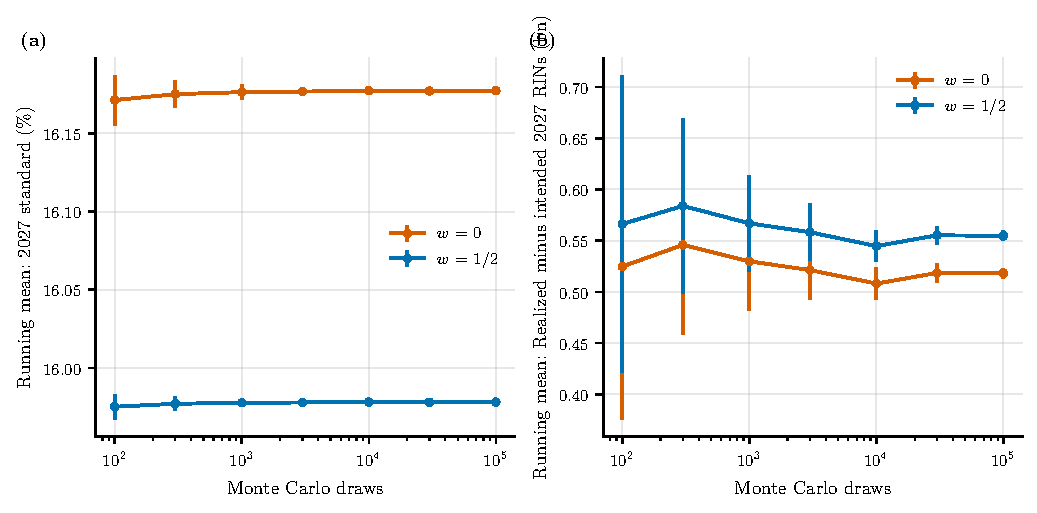
\includegraphics[width=\textwidth]{si_convergence}
\caption{Running means of the 2027 standard and of the realized-minus-intended 2027 obligation with 95~percent Monte Carlo error bars, for $w=0$ and $w=1/2$.}\label{fig:conv}\end{figure}

\section{Sensitivity indices and empirical distributions}

\begin{figure}[htbp]\centering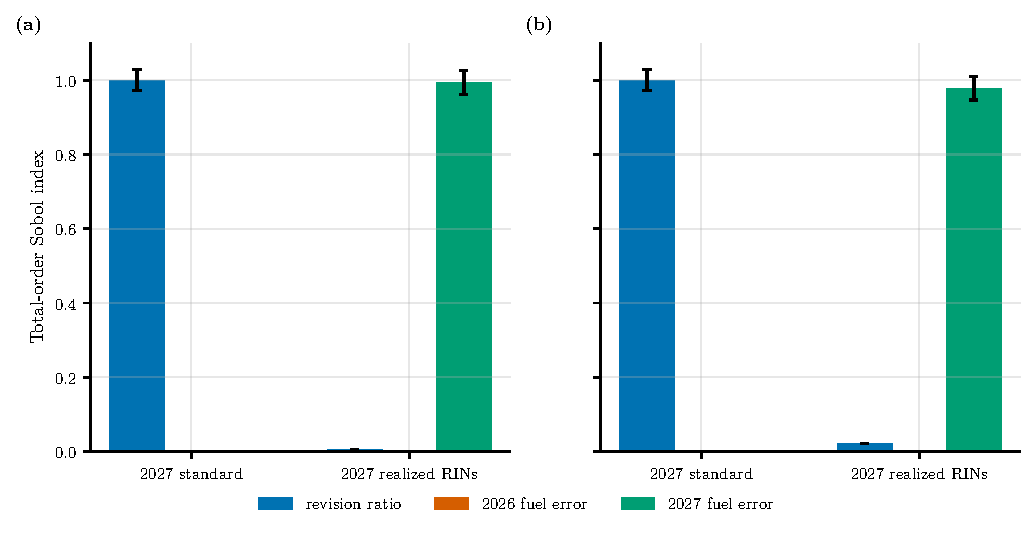
\includegraphics[width=\textwidth]{si_sobol}
\caption{Total-order Sobol indices with bootstrap intervals for the 2027 standard and the realized 2027 obligation: (a)~equal split ($w = 1/2$), (b)~2027 approach ($w = 0$).}\end{figure}

\begin{figure}[htbp]\centering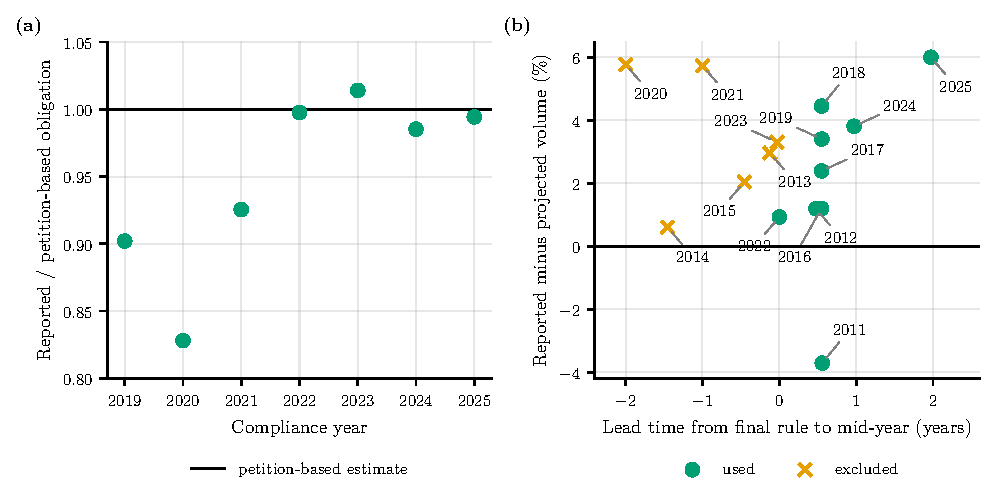
\includegraphics[width=\textwidth]{si_distributions}
\caption{(a)~Ratio of reported to petition-based exempted obligation by compliance year. (b)~Reported minus projected non-renewable gasoline-plus-diesel volume against lead time; crosses mark rules published after the middle of the compliance year or later revised, which are excluded.}\end{figure}

\section{Cross-check against a secondary analysis}

As an independent check of derived quantities, the obligation that the additional 2025 exempted fuel (\valcrossCheckExtraExemptFuel{} billion gallons above the Set~2 projection) would remove if it were not reallocated is \valcrossCheckBbdReduction{} billion RINs for biomass-based diesel and \valcrossCheckRfReduction{} billion RINs for total renewable fuel at the 2026 standards. The secondary analysis of \citet{hubbs2026farmdoc} states about 0.3 and nearly 1 billion RINs for the same quantities, and quotes the 2025 exempted volume (13.38 billion gallons), the exempted obligation (1.76 billion RINs) and the additional volume (0.77 billion RINs) used here. That analysis is cited only as a cross-check and supplies no parameter.

\section{Sensitivity configurations}

Two additional configurations were run with identical seeds: a uniform $\pm 20$~percent revision distribution (an assumption, not data) and independent fuel-use errors for 2026 and 2027. The uniform assumption raises the standard deviation of the 2027 standard under the 2027 approach from \valstdSdSecondAllSecond{} to \valsensUniformStdSdSecondAllSecond{} points and the expected absolute revision from \valrevisionMeanAbsSecondAllSecond{} to \valsensUniformRevisionMeanAbsSecondAllSecond{} points; independent fuel-use errors leave the single-year distributions essentially unchanged (standard deviation of the realized-minus-intended 2027 obligation \valsensIndependentFuelRealizedMinusIntendedSdSecondAllSecond{} against \valrealizedMinusIntendedSdSecondAllSecond{} billion RINs). Results are in \texttt{results/sensitivity\_uniform\_revision} and \texttt{results/sensitivity\_independent\_fuel\_errors}.

\section{Full transcription}

\scriptsize
\begin{longtable}{p{2.3cm}p{0.7cm}p{1.0cm}p{2.6cm}rp{1.7cm}p{4.6cm}}
\caption{Transcribed values with sources (entry A).}\\
\toprule
Table & Year & Category & Variable & Value & Unit & Source, locator \\
\midrule
\endfirsthead
\toprule
Table & Year & Category & Variable & Value & Unit & Source, locator \\
\midrule
\endhead
\bottomrule
\endfoot
set2\_inputs & 2026 & CB & RFV & 1.36 & billion RINs & docket\_0789, p. 1 table \\
set2\_inputs & 2026 & BBD & RFV & 8.86 & billion RINs & docket\_0789, p. 1 table \\
set2\_inputs & 2026 & AB & RFV & 10.82 & billion RINs & docket\_0789, p. 1 table \\
set2\_inputs & 2026 & RF & RFV & 25.82 & billion RINs & docket\_0789, p. 1 table \\
set2\_inputs & 2026 &  & G & 140.07 & billion gallons & docket\_0789, p. 1 table \\
set2\_inputs & 2026 &  & D & 60.46 & billion gallons & docket\_0789, p. 1 table \\
set2\_inputs & 2026 &  & RG & 14.85 & billion gallons & docket\_0789, p. 1 table \\
set2\_inputs & 2026 &  & RD & 5.11 & billion gallons & docket\_0789, p. 1 table \\
set2\_inputs & 2026 &  & GE & 4.35 & billion gallons & docket\_0789, p. 1 table \\
set2\_inputs & 2026 &  & DE & 3.20 & billion gallons & docket\_0789, p. 1 table \\
set2\_inputs & 2027 & CB & RFV & 1.43 & billion RINs & docket\_0789, p. 1 table \\
set2\_inputs & 2027 & BBD & RFV & 8.95 & billion RINs & docket\_0789, p. 1 table \\
set2\_inputs & 2027 & AB & RFV & 10.98 & billion RINs & docket\_0789, p. 1 table \\
set2\_inputs & 2027 & RF & RFV & 25.98 & billion RINs & docket\_0789, p. 1 table \\
set2\_inputs & 2027 &  & G & 139.18 & billion gallons & docket\_0789, p. 1 table \\
set2\_inputs & 2027 &  & D & 59.72 & billion gallons & docket\_0789, p. 1 table \\
set2\_inputs & 2027 &  & RG & 14.85 & billion gallons & docket\_0789, p. 1 table \\
set2\_inputs & 2027 &  & RD & 5.26 & billion gallons & docket\_0789, p. 1 table \\
set2\_inputs & 2027 &  & GE & 4.35 & billion gallons & docket\_0789, p. 1 table \\
set2\_inputs & 2027 &  & DE & 3.20 & billion gallons & docket\_0789, p. 1 table \\
set2\_aeo & 2026 &  & gasoline\_mbd & 8.94 & million barrels per day & docket\_0789, p. 2 Gasoline Projections \\
set2\_aeo & 2027 &  & gasoline\_mbd & 8.88 & million barrels per day & docket\_0789, p. 2 Gasoline Projections \\
set2\_aeo & 2026 &  & ethanol\_quad & 1.23 & quadrillion Btu & docket\_0789, p. 2 Gasoline Projections \\
set2\_aeo & 2027 &  & ethanol\_quad & 1.23 & quadrillion Btu & docket\_0789, p. 2 Gasoline Projections \\
set2\_aeo &  &  & gasoline\_adjustment & 0.022 & fraction & docket\_0789, p. 2 Adjustment Factor \\
set2\_aeo & 2026 &  & obligated\_gasoline & 125.22 & billion gallons & docket\_0789, p. 2 Total Obligated Gasoline \\
set2\_aeo & 2027 &  & obligated\_gasoline & 124.33 & billion gallons & docket\_0789, p. 2 Total Obligated Gasoline \\
set2\_aeo & 2026 &  & distillate\_mbd & 4.25 & million barrels per day & docket\_0789, p. 3 Diesel Projections \\
set2\_aeo & 2027 &  & distillate\_mbd & 4.20 & million barrels per day & docket\_0789, p. 3 Diesel Projections \\
set2\_aeo & 2026 &  & biodiesel\_mbd & 0.10 & million barrels per day & docket\_0789, p. 3 Diesel Projections \\
set2\_aeo & 2027 &  & biodiesel\_mbd & 0.10 & million barrels per day & docket\_0789, p. 3 Diesel Projections \\
set2\_aeo & 2026 &  & renewable\_diesel\_mbd & 0.25 & million barrels per day & docket\_0789, p. 3 Diesel Projections \\
set2\_aeo & 2027 &  & renewable\_diesel\_mbd & 0.24 & million barrels per day & docket\_0789, p. 3 Diesel Projections \\
set2\_aeo & 2026 &  & other\_biofuels\_mbd & 0.01 & million barrels per day & docket\_0789, p. 3 Diesel Projections \\
set2\_aeo & 2027 &  & other\_biofuels\_mbd & 0.03 & million barrels per day & docket\_0789, p. 3 Diesel Projections \\
set2\_aeo &  &  & diesel\_adjustment & -0.073 & fraction & docket\_0789, p. 3 Adjustment Factor \\
set2\_aeo & 2026 &  & obligated\_diesel & 55.35 & billion gallons & docket\_0789, p. 3 Total Obligated Diesel \\
set2\_aeo & 2027 &  & obligated\_diesel & 54.46 & billion gallons & docket\_0789, p. 3 Total Obligated Diesel \\
set2\_aeo &  &  & ethanol\_hhv & 3.563 & million Btu per barrel & docket\_0789, p. 4 Energy Content \\
srerv & 2026 & BBD & set2 & 0.21 & billion RINs & fr\_2026\_21155, Table IV-1 \\
srerv & 2026 & AB & set2 & 0.28 & billion RINs & fr\_2026\_21155, Table IV-1 \\
srerv & 2026 & RF & set2 & 0.99 & billion RINs & fr\_2026\_21155, Table IV-1 \\
srerv & 2027 & BBD & set2 & 0.25 & billion RINs & fr\_2026\_21155, Table IV-1 \\
srerv & 2027 & AB & set2 & 0.34 & billion RINs & fr\_2026\_21155, Table IV-1 \\
srerv & 2027 & RF & set2 & 1.04 & billion RINs & fr\_2026\_21155, Table IV-1 \\
srerv & 2026 & BBD & equal & 0.30 & billion RINs & fr\_2026\_21155, Table IV-1 \\
srerv & 2026 & AB & equal & 0.40 & billion RINs & fr\_2026\_21155, Table IV-1 \\
srerv & 2026 & RF & equal & 1.37 & billion RINs & fr\_2026\_21155, Table IV-1 \\
srerv & 2027 & BBD & equal & 0.34 & billion RINs & fr\_2026\_21155, Table IV-1 \\
srerv & 2027 & AB & equal & 0.47 & billion RINs & fr\_2026\_21155, Table IV-1 \\
srerv & 2027 & RF & equal & 1.43 & billion RINs & fr\_2026\_21155, Table IV-1 \\
srerv & 2026 & BBD & all2027 & 0.21 & billion RINs & fr\_2026\_21155, Table IV-1 \\
srerv & 2026 & AB & all2027 & 0.28 & billion RINs & fr\_2026\_21155, Table IV-1 \\
srerv & 2026 & RF & all2027 & 0.99 & billion RINs & fr\_2026\_21155, Table IV-1 \\
srerv & 2027 & BBD & all2027 & 0.43 & billion RINs & fr\_2026\_21155, Table IV-1 \\
srerv & 2027 & AB & all2027 & 0.59 & billion RINs & fr\_2026\_21155, Table IV-1 \\
srerv & 2027 & RF & all2027 & 1.81 & billion RINs & fr\_2026\_21155, Table IV-1 \\
srerv\_set2\_million & 2026 & BBD & set2 & 210 & million RINs & fr\_2026\_06275, Table IV.C-3 (91 FR 16440) \\
srerv\_set2\_million & 2026 & AB & set2 & 280 & million RINs & fr\_2026\_06275, Table IV.C-3 (91 FR 16440) \\
srerv\_set2\_million & 2026 & RF & set2 & 990 & million RINs & fr\_2026\_06275, Table IV.C-3 (91 FR 16440) \\
srerv\_set2\_million & 2027 & BBD & set2 & 250 & million RINs & fr\_2026\_06275, Table IV.C-3 (91 FR 16440) \\
srerv\_set2\_million & 2027 & AB & set2 & 340 & million RINs & fr\_2026\_06275, Table IV.C-3 (91 FR 16440) \\
srerv\_set2\_million & 2027 & RF & set2 & 1040 & million RINs & fr\_2026\_06275, Table IV.C-3 (91 FR 16440) \\
standards & 2026 & CB & set2 & 0.79 & percent & fr\_2026\_06275, Table V.D-1 (91 FR 16441) \\
standards & 2026 & BBD & set2 & 5.24 & percent & fr\_2026\_06275, Table V.D-1 (91 FR 16441) \\
standards & 2026 & AB & set2 & 6.42 & percent & fr\_2026\_06275, Table V.D-1 (91 FR 16441) \\
standards & 2026 & RF & set2 & 15.50 & percent & fr\_2026\_06275, Table V.D-1 (91 FR 16441) \\
standards & 2027 & CB & set2 & 0.84 & percent & fr\_2026\_06275, Table V.D-1 (91 FR 16441) \\
standards & 2027 & BBD & set2 & 5.37 & percent & fr\_2026\_06275, Table V.D-1 (91 FR 16441) \\
standards & 2027 & AB & set2 & 6.61 & percent & fr\_2026\_06275, Table V.D-1 (91 FR 16441) \\
standards & 2027 & RF & set2 & 15.78 & percent & fr\_2026\_06275, Table V.D-1 (91 FR 16441) \\
standards & 2026 & CB & equal & 0.79 & percent & fr\_2026\_21155, Table VI-1 \\
standards & 2026 & BBD & equal & 5.29 & percent & fr\_2026\_21155, Table V-1 \\
standards & 2026 & AB & equal & 6.48 & percent & fr\_2026\_21155, Table V-1 \\
standards & 2026 & RF & equal & 15.71 & percent & fr\_2026\_21155, Table V-1 \\
standards & 2027 & CB & equal & 0.84 & percent & fr\_2026\_21155, Table VI-1 \\
standards & 2027 & BBD & equal & 5.43 & percent & fr\_2026\_21155, Table V-1 \\
standards & 2027 & AB & equal & 6.69 & percent & fr\_2026\_21155, Table V-1 \\
standards & 2027 & RF & equal & 16.01 & percent & fr\_2026\_21155, Table V-1 \\
standards & 2026 & CB & all2027 & 0.79 & percent & fr\_2026\_21155, Table VI-1 \\
standards & 2026 & BBD & all2027 & 5.24 & percent & fr\_2026\_21155, Table V-1 \\
standards & 2026 & AB & all2027 & 6.42 & percent & fr\_2026\_21155, Table V-1 \\
standards & 2026 & RF & all2027 & 15.50 & percent & fr\_2026\_21155, Table V-1 \\
standards & 2027 & CB & all2027 & 0.84 & percent & fr\_2026\_21155, Table VI-1 \\
standards & 2027 & BBD & all2027 & 5.48 & percent & fr\_2026\_21155, Table V-1 \\
standards & 2027 & AB & all2027 & 6.76 & percent & fr\_2026\_21155, Table V-1 \\
standards & 2027 & RF & all2027 & 16.23 & percent & fr\_2026\_21155, Table V-1 \\
standards & 2026 & CB & no\_srerv & 0.79 & percent & docket\_0790, p. 1 table \\
standards & 2026 & BBD & no\_srerv & 5.12 & percent & docket\_0790, p. 1 table \\
standards & 2026 & AB & no\_srerv & 6.25 & percent & docket\_0790, p. 1 table \\
standards & 2026 & RF & no\_srerv & 14.92 & percent & docket\_0790, p. 1 table \\
standards & 2027 & CB & no\_srerv & 0.84 & percent & docket\_0790, p. 1 table \\
standards & 2027 & BBD & no\_srerv & 5.23 & percent & docket\_0790, p. 1 table \\
standards & 2027 & AB & no\_srerv & 6.41 & percent & docket\_0790, p. 1 table \\
standards & 2027 & RF & no\_srerv & 15.17 & percent & docket\_0790, p. 1 table \\
set2\_exempted\_fuel & 2022 &  & gasoline & 3.97 & billion gallons & fr\_2026\_06275, Table IV.C-1 (91 FR 16439) \\
set2\_exempted\_fuel & 2022 &  & diesel & 3.08 & billion gallons & fr\_2026\_06275, Table IV.C-1 (91 FR 16439) \\
set2\_exempted\_fuel & 2022 &  & total & 7.06 & billion gallons & fr\_2026\_06275, Table IV.C-1 (91 FR 16439) \\
set2\_exempted\_fuel & 2023 &  & gasoline & 4.58 & billion gallons & fr\_2026\_06275, Table IV.C-1 (91 FR 16439) \\
set2\_exempted\_fuel & 2023 &  & diesel & 3.22 & billion gallons & fr\_2026\_06275, Table IV.C-1 (91 FR 16439) \\
set2\_exempted\_fuel & 2023 &  & total & 7.79 & billion gallons & fr\_2026\_06275, Table IV.C-1 (91 FR 16439) \\
set2\_exempted\_fuel & 2024 &  & gasoline & 4.50 & billion gallons & fr\_2026\_06275, Table IV.C-1 (91 FR 16439) \\
set2\_exempted\_fuel & 2024 &  & diesel & 3.29 & billion gallons & fr\_2026\_06275, Table IV.C-1 (91 FR 16439) \\
set2\_exempted\_fuel & 2024 &  & total & 7.78 & billion gallons & fr\_2026\_06275, Table IV.C-1 (91 FR 16439) \\
set2\_exempted\_fuel & 2025 &  & gasoline & 4.35 & billion gallons & fr\_2026\_06275, Table IV.C-1 (91 FR 16439) \\
set2\_exempted\_fuel & 2025 &  & diesel & 3.20 & billion gallons & fr\_2026\_06275, Table IV.C-1 (91 FR 16439) \\
set2\_exempted\_fuel & 2025 &  & total & 7.55 & billion gallons & fr\_2026\_06275, Table IV.C-1 (91 FR 16439) \\
set2\_exempted\_rvo & 2023 & CB & standard & 0.48 & percent & fr\_2026\_06275, Table IV.C-2 (91 FR 16439) \\
set2\_exempted\_rvo & 2023 & BBD & standard & 2.58 & percent & fr\_2026\_06275, Table IV.C-2 (91 FR 16439) \\
set2\_exempted\_rvo & 2023 & AB & standard & 3.39 & percent & fr\_2026\_06275, Table IV.C-2 (91 FR 16439) \\
set2\_exempted\_rvo & 2023 & RF & standard & 11.96 & percent & fr\_2026\_06275, Table IV.C-2 (91 FR 16439) \\
set2\_exempted\_rvo & 2024 & CB & standard & 0.59 & percent & fr\_2026\_06275, Table IV.C-2 (91 FR 16439) \\
set2\_exempted\_rvo & 2024 & BBD & standard & 2.82 & percent & fr\_2026\_06275, Table IV.C-2 (91 FR 16439) \\
set2\_exempted\_rvo & 2024 & AB & standard & 3.79 & percent & fr\_2026\_06275, Table IV.C-2 (91 FR 16439) \\
set2\_exempted\_rvo & 2024 & RF & standard & 12.50 & percent & fr\_2026\_06275, Table IV.C-2 (91 FR 16439) \\
set2\_exempted\_rvo & 2025 & CB & standard & 0.71 & percent & fr\_2026\_06275, Table IV.C-2 (91 FR 16439) \\
set2\_exempted\_rvo & 2025 & BBD & standard & 3.15 & percent & fr\_2026\_06275, Table IV.C-2 (91 FR 16439) \\
set2\_exempted\_rvo & 2025 & AB & standard & 4.31 & percent & fr\_2026\_06275, Table IV.C-2 (91 FR 16439) \\
set2\_exempted\_rvo & 2025 & RF & standard & 13.13 & percent & fr\_2026\_06275, Table IV.C-2 (91 FR 16439) \\
set2\_exempted\_rvo & 2023 & CB & ervo & 40 & million RINs & fr\_2026\_06275, Table IV.C-2 (91 FR 16439) \\
set2\_exempted\_rvo & 2023 & BBD & ervo & 200 & million RINs & fr\_2026\_06275, Table IV.C-2 (91 FR 16439) \\
set2\_exempted\_rvo & 2023 & AB & ervo & 260 & million RINs & fr\_2026\_06275, Table IV.C-2 (91 FR 16439) \\
set2\_exempted\_rvo & 2023 & RF & ervo & 930 & million RINs & fr\_2026\_06275, Table IV.C-2 (91 FR 16439) \\
set2\_exempted\_rvo & 2024 & CB & ervo & 50 & million RINs & fr\_2026\_06275, Table IV.C-2 (91 FR 16439) \\
set2\_exempted\_rvo & 2024 & BBD & ervo & 220 & million RINs & fr\_2026\_06275, Table IV.C-2 (91 FR 16439) \\
set2\_exempted\_rvo & 2024 & AB & ervo & 300 & million RINs & fr\_2026\_06275, Table IV.C-2 (91 FR 16439) \\
set2\_exempted\_rvo & 2024 & RF & ervo & 970 & million RINs & fr\_2026\_06275, Table IV.C-2 (91 FR 16439) \\
set2\_exempted\_rvo & 2025 & CB & ervo & 50 & million RINs & fr\_2026\_06275, Table IV.C-2 (91 FR 16439) \\
set2\_exempted\_rvo & 2025 & BBD & ervo & 240 & million RINs & fr\_2026\_06275, Table IV.C-2 (91 FR 16439) \\
set2\_exempted\_rvo & 2025 & AB & ervo & 330 & million RINs & fr\_2026\_06275, Table IV.C-2 (91 FR 16439) \\
set2\_exempted\_rvo & 2025 & RF & ervo & 990 & million RINs & fr\_2026\_06275, Table IV.C-2 (91 FR 16439) \\
set2\_exempted\_rvo &  & CB & ervo\_total & 140 & million RINs & fr\_2026\_06275, Table IV.C-2 (91 FR 16439) \\
set2\_exempted\_rvo &  & BBD & ervo\_total & 660 & million RINs & fr\_2026\_06275, Table IV.C-2 (91 FR 16439) \\
set2\_exempted\_rvo &  & AB & ervo\_total & 890 & million RINs & fr\_2026\_06275, Table IV.C-2 (91 FR 16439) \\
set2\_exempted\_rvo &  & RF & ervo\_total & 2890 & million RINs & fr\_2026\_06275, Table IV.C-2 (91 FR 16439) \\
set2\_total\_applicable & 2026 & CB & total & 1.36 & billion RINs & fr\_2026\_06275, Table V.A-1 (91 FR 16440) \\
set2\_total\_applicable & 2026 & BBD & total & 9.07 & billion RINs & fr\_2026\_06275, Table V.A-1 (91 FR 16440) \\
set2\_total\_applicable & 2026 & AB & total & 11.10 & billion RINs & fr\_2026\_06275, Table V.A-1 (91 FR 16440) \\
set2\_total\_applicable & 2026 & RF & total & 26.81 & billion RINs & fr\_2026\_06275, Table V.A-1 (91 FR 16440) \\
set2\_total\_applicable & 2027 & CB & total & 1.43 & billion RINs & fr\_2026\_06275, Table V.A-1 (91 FR 16440) \\
set2\_total\_applicable & 2027 & BBD & total & 9.20 & billion RINs & fr\_2026\_06275, Table V.A-1 (91 FR 16440) \\
set2\_total\_applicable & 2027 & AB & total & 11.32 & billion RINs & fr\_2026\_06275, Table V.A-1 (91 FR 16440) \\
set2\_total\_applicable & 2027 & RF & total & 27.02 & billion RINs & fr\_2026\_06275, Table V.A-1 (91 FR 16440) \\
proposal\_2025\_sre & 2025 &  & exempted\_fuel\_volume & 13.38 & billion gallons & fr\_2026\_21155, Section II \\
proposal\_2025\_sre & 2025 &  & actual\_exempted\_rvo & 1.76 & billion RINs & fr\_2026\_21155, Section I \\
proposal\_2025\_sre & 2025 &  & projected\_exempted\_rvo & 0.99 & billion RINs & fr\_2026\_21155, Section I \\
proposal\_2025\_sre & 2025 &  & additional\_exempted\_rvo & 0.77 & billion RINs & fr\_2026\_21155, Section I \\
proposal\_2025\_sre & 2025 &  & projected\_exempted\_fuel\_volume & 7.55 & billion gallons & fr\_2026\_21155, Section II \\
proposal\_2025\_sre & 2025 &  & petitions & 34 & count & fr\_2026\_21155, Section II \\
proposal\_2025\_sre & 2025 &  & full\_exemptions & 18 & count & fr\_2026\_21155, Section II \\
proposal\_2025\_sre & 2025 &  & partial\_exemptions & 11 & count & fr\_2026\_21155, Section II \\
proposal\_2025\_sre & 2025 &  & denials & 3 & count & fr\_2026\_21155, Section II \\
proposal\_2025\_sre & 2025 &  & ineligible & 2 & count & fr\_2026\_21155, Section II \\
proposal\_2025\_sre & 2025 &  & reallocation\_share\_set2 & 0.70 & fraction & fr\_2026\_21155, Section I \\
proposal\_2025\_sre & 2025 &  & reallocation\_share\_additional & 1.00 & fraction & fr\_2026\_21155, Section I \\
proposal\_2025\_sre & 2026 &  & renewable\_fuel\_volume & 24.02 & billion RINs & fr\_2026\_21155, Section VI \\
proposal\_2025\_sre & 2027 &  & renewable\_fuel\_volume & 24.46 & billion RINs & fr\_2026\_21155, Section VI \\
table\_vi1 & 2026 & CB & existing & 0.79 & percent & fr\_2026\_21155, Table VI-1 \\
table\_vi1 & 2027 & CB & existing & 0.84 & percent & fr\_2026\_21155, Table VI-1 \\
table\_vi1 & 2026 & BBD & existing & 5.24 & percent & fr\_2026\_21155, Table VI-1 \\
table\_vi1 & 2027 & BBD & existing & 5.37 & percent & fr\_2026\_21155, Table VI-1 \\
table\_vi1 & 2026 & OA & existing & 0.39 & percent & fr\_2026\_21155, Table VI-1 \\
table\_vi1 & 2027 & OA & existing & 0.40 & percent & fr\_2026\_21155, Table VI-1 \\
table\_vi1 & 2026 & CONV & existing & 9.08 & percent & fr\_2026\_21155, Table VI-1 \\
table\_vi1 & 2027 & CONV & existing & 9.17 & percent & fr\_2026\_21155, Table VI-1 \\
table\_vi1 & 2026 & RINCOST & existing & 27.5 & cents per gallon & fr\_2026\_21155, Table VI-1 \\
table\_vi1 & 2027 & RINCOST & existing & 28.0 & cents per gallon & fr\_2026\_21155, Table VI-1 \\
table\_vi1 & 2026 & GASOLINE & existing & 6.8 & cents per gallon & fr\_2026\_21155, Table VI-1 \\
table\_vi1 & 2027 & GASOLINE & existing & 7.3 & cents per gallon & fr\_2026\_21155, Table VI-1 \\
table\_vi1 & 2026 & DIESEL & existing & 18.6 & cents per gallon & fr\_2026\_21155, Table VI-1 \\
table\_vi1 & 2027 & DIESEL & existing & 21.0 & cents per gallon & fr\_2026\_21155, Table VI-1 \\
table\_vi1 & 2026 & CB & equal & 0.79 & percent & fr\_2026\_21155, Table VI-1 \\
table\_vi1 & 2027 & CB & equal & 0.84 & percent & fr\_2026\_21155, Table VI-1 \\
table\_vi1 & 2026 & BBD & equal & 5.29 & percent & fr\_2026\_21155, Table VI-1 \\
table\_vi1 & 2027 & BBD & equal & 5.43 & percent & fr\_2026\_21155, Table VI-1 \\
table\_vi1 & 2026 & OA & equal & 0.40 & percent & fr\_2026\_21155, Table VI-1 \\
table\_vi1 & 2027 & OA & equal & 0.42 & percent & fr\_2026\_21155, Table VI-1 \\
table\_vi1 & 2026 & CONV & equal & 9.23 & percent & fr\_2026\_21155, Table VI-1 \\
table\_vi1 & 2027 & CONV & equal & 9.32 & percent & fr\_2026\_21155, Table VI-1 \\
table\_vi1 & 2026 & RINCOST & equal & 27.9 & cents per gallon & fr\_2026\_21155, Table VI-1 \\
table\_vi1 & 2027 & RINCOST & equal & 28.4 & cents per gallon & fr\_2026\_21155, Table VI-1 \\
table\_vi1 & 2026 & GASOLINE & equal & 7.2 & cents per gallon & fr\_2026\_21155, Table VI-1 \\
table\_vi1 & 2027 & GASOLINE & equal & 7.6 & cents per gallon & fr\_2026\_21155, Table VI-1 \\
table\_vi1 & 2026 & DIESEL & equal & 19.0 & cents per gallon & fr\_2026\_21155, Table VI-1 \\
table\_vi1 & 2027 & DIESEL & equal & 21.4 & cents per gallon & fr\_2026\_21155, Table VI-1 \\
table\_vi1 & 2026 & CB & all2027 & 0.79 & percent & fr\_2026\_21155, Table VI-1 \\
table\_vi1 & 2027 & CB & all2027 & 0.84 & percent & fr\_2026\_21155, Table VI-1 \\
table\_vi1 & 2026 & BBD & all2027 & 5.24 & percent & fr\_2026\_21155, Table VI-1 \\
table\_vi1 & 2027 & BBD & all2027 & 5.48 & percent & fr\_2026\_21155, Table VI-1 \\
table\_vi1 & 2026 & OA & all2027 & 0.39 & percent & fr\_2026\_21155, Table VI-1 \\
table\_vi1 & 2027 & OA & all2027 & 0.44 & percent & fr\_2026\_21155, Table VI-1 \\
table\_vi1 & 2026 & CONV & all2027 & 9.08 & percent & fr\_2026\_21155, Table VI-1 \\
table\_vi1 & 2027 & CONV & all2027 & 9.47 & percent & fr\_2026\_21155, Table VI-1 \\
table\_vi1 & 2026 & RINCOST & all2027 & 27.5 & cents per gallon & fr\_2026\_21155, Table VI-1 \\
table\_vi1 & 2027 & RINCOST & all2027 & 28.8 & cents per gallon & fr\_2026\_21155, Table VI-1 \\
table\_vi1 & 2026 & GASOLINE & all2027 & 6.8 & cents per gallon & fr\_2026\_21155, Table VI-1 \\
table\_vi1 & 2027 & GASOLINE & all2027 & 8.0 & cents per gallon & fr\_2026\_21155, Table VI-1 \\
table\_vi1 & 2026 & DIESEL & all2027 & 18.6 & cents per gallon & fr\_2026\_21155, Table VI-1 \\
table\_vi1 & 2027 & DIESEL & all2027 & 21.8 & cents per gallon & fr\_2026\_21155, Table VI-1 \\
price\_impact\_relative & 2026 & GASOLINE & equal & 0.4 & cents per gallon & docket\_0961, Table 2 \\
price\_impact\_relative & 2027 & GASOLINE & equal & 0.4 & cents per gallon & docket\_0961, Table 2 \\
price\_impact\_relative & 2026 & DIESEL & equal & 0.4 & cents per gallon & docket\_0961, Table 2 \\
price\_impact\_relative & 2027 & DIESEL & equal & 0.4 & cents per gallon & docket\_0961, Table 2 \\
price\_impact\_relative & 2026 & GASOLINE & all2027 & 0.0 & cents per gallon & docket\_0961, Table 2 \\
price\_impact\_relative & 2027 & GASOLINE & all2027 & 0.8 & cents per gallon & docket\_0961, Table 2 \\
price\_impact\_relative & 2026 & DIESEL & all2027 & 0.0 & cents per gallon & docket\_0961, Table 2 \\
price\_impact\_relative & 2027 & DIESEL & all2027 & 0.8 & cents per gallon & docket\_0961, Table 2 \\
rin\_prices &  & D3 & set2 & 2.40 & dollars per RIN & docket\_0961, Table 1 \\
rin\_prices &  & D4 & set2 & 0.95 & dollars per RIN & docket\_0961, Table 1 \\
rin\_prices &  & D5 & set2 & 0.99 & dollars per RIN & docket\_0961, Table 1 \\
rin\_prices &  & D6 & set2 & 0.91 & dollars per RIN & docket\_0961, Table 1 \\
rin\_prices &  & D3 & proposal & 2.45 & dollars per RIN & docket\_0961, Table 1 \\
rin\_prices &  & D4 & proposal & 1.74 & dollars per RIN & docket\_0961, Table 1 \\
rin\_prices &  & D5 & proposal & 1.94 & dollars per RIN & docket\_0961, Table 1 \\
rin\_prices &  & D6 & proposal & 1.73 & dollars per RIN & docket\_0961, Table 1 \\
fuel\_cost\_average & 2026 & GASOLINE & no\_rfs & 2.15 & dollars per gallon & docket\_0961, Table A-9 \\
fuel\_cost\_average & 2027 & GASOLINE & no\_rfs & 2.09 & dollars per gallon & docket\_0961, Table A-9 \\
fuel\_cost\_average & 2026 & GASOLINE & existing & 2.22 & dollars per gallon & docket\_0961, Table A-9 \\
fuel\_cost\_average & 2027 & GASOLINE & existing & 2.16 & dollars per gallon & docket\_0961, Table A-9 \\
fuel\_cost\_average & 2026 & GASOLINE & equal & 2.22 & dollars per gallon & docket\_0961, Table A-10 \\
fuel\_cost\_average & 2027 & GASOLINE & equal & 2.17 & dollars per gallon & docket\_0961, Table A-10 \\
fuel\_cost\_average & 2026 & GASOLINE & all2027 & 2.22 & dollars per gallon & docket\_0961, Table A-11 \\
fuel\_cost\_average & 2027 & GASOLINE & all2027 & 2.17 & dollars per gallon & docket\_0961, Table A-11 \\
fuel\_cost\_average & 2026 & DIESEL & no\_rfs & 2.67 & dollars per gallon & docket\_0961, Table B-9 \\
fuel\_cost\_average & 2027 & DIESEL & no\_rfs & 2.64 & dollars per gallon & docket\_0961, Table B-9 \\
fuel\_cost\_average & 2026 & DIESEL & existing & 2.85 & dollars per gallon & docket\_0961, Table B-9 \\
fuel\_cost\_average & 2027 & DIESEL & existing & 2.85 & dollars per gallon & docket\_0961, Table B-9 \\
fuel\_cost\_average & 2026 & DIESEL & equal & 2.86 & dollars per gallon & docket\_0961, Table B-10 \\
fuel\_cost\_average & 2027 & DIESEL & equal & 2.85 & dollars per gallon & docket\_0961, Table B-10 \\
fuel\_cost\_average & 2026 & DIESEL & all2027 & 2.85 & dollars per gallon & docket\_0961, Table B-11 \\
fuel\_cost\_average & 2027 & DIESEL & all2027 & 2.85 & dollars per gallon & docket\_0961, Table B-11 \\
ria\_srerv\_share & 2026 & BBD & standard\_share & 0.12 & percent & ria\_420r26011, Table 10.5.4-1 (p. 416) \\
ria\_srerv\_share & 2027 & BBD & standard\_share & 0.14 & percent & ria\_420r26011, Table 10.5.4-1 (p. 416) \\
ria\_srerv\_share & 2026 & OA & standard\_share & 0.05 & percent & ria\_420r26011, Table 10.5.4-1 (p. 416) \\
ria\_srerv\_share & 2027 & OA & standard\_share & 0.06 & percent & ria\_420r26011, Table 10.5.4-1 (p. 416) \\
ria\_srerv\_share & 2026 & CONV & standard\_share & 0.41 & percent & ria\_420r26011, Table 10.5.4-1 (p. 416) \\
ria\_srerv\_share & 2027 & CONV & standard\_share & 0.41 & percent & ria\_420r26011, Table 10.5.4-1 (p. 416) \\
ria\_srerv\_share & 2026 & RF & price\_impact & 0.5 & cents per gallon & ria\_420r26011, Table 10.5.4-1 (p. 416) \\
ria\_srerv\_share & 2027 & RF & price\_impact & 0.6 & cents per gallon & ria\_420r26011, Table 10.5.4-1 (p. 416) \\
carryover\_2024 &  & CB & carryover & 72428101 & RINs & ria\_420r26011, Table 1.8.1-4 (p. 36) \\
carryover\_2024 &  & NCA & carryover & 2513591893 & RINs & ria\_420r26011, Table 1.8.1-4 (p. 36) \\
carryover\_2024 &  & CONV & carryover & 1296096353 & RINs & ria\_420r26011, Table 1.8.1-4 (p. 36) \\
carryover\_2024 &  & RF & carryover & 3882116347 & RINs & ria\_420r26011, Table 1.8.1-4 (p. 36) \\
carryover\_2024 &  & CB & deficit & 55110052 & RINs & ria\_420r26011, Table 1.8.1-4 (p. 36) \\
carryover\_2024 &  & NCA & deficit & 0 & RINs & ria\_420r26011, Table 1.8.1-4 (p. 36) \\
carryover\_2024 &  & CONV & deficit & 228735586 & RINs & ria\_420r26011, Table 1.8.1-4 (p. 36) \\
carryover\_2024 &  & RF & deficit & 280333003 & RINs & ria\_420r26011, Table 1.8.1-4 (p. 36) \\
carryover\_2024 &  & CB & effective & 17318049 & RINs & ria\_420r26011, Table 1.8.1-4 (p. 36) \\
carryover\_2024 &  & NCA & effective & 2513591893 & RINs & ria\_420r26011, Table 1.8.1-4 (p. 36) \\
carryover\_2024 &  & CONV & effective & 1067360767 & RINs & ria\_420r26011, Table 1.8.1-4 (p. 36) \\
carryover\_2024 &  & RF & effective & 3601783344 & RINs & ria\_420r26011, Table 1.8.1-4 (p. 36) \\
rins\_retired\_2024 & 2023 & D3 & retired & 69969240 & RINs & ria\_420r26011, Table 1.8.1-1 (p. 34) \\
rins\_retired\_2024 & 2024 & D3 & retired & 939117670 & RINs & ria\_420r26011, Table 1.8.1-1 (p. 34) \\
rins\_retired\_2024 & 2023 & D4 & retired & 1104174020 & RINs & ria\_420r26011, Table 1.8.1-1 (p. 34) \\
rins\_retired\_2024 & 2024 & D4 & retired & 6612812357 & RINs & ria\_420r26011, Table 1.8.1-1 (p. 34) \\
rins\_retired\_2024 & 2023 & D5 & retired & 18005685 & RINs & ria\_420r26011, Table 1.8.1-1 (p. 34) \\
rins\_retired\_2024 & 2024 & D5 & retired & 226676380 & RINs & ria\_420r26011, Table 1.8.1-1 (p. 34) \\
rins\_retired\_2024 & 2023 & D6 & retired & 1274536953 & RINs & ria\_420r26011, Table 1.8.1-1 (p. 34) \\
rins\_retired\_2024 & 2024 & D6 & retired & 13562182158 & RINs & ria\_420r26011, Table 1.8.1-1 (p. 34) \\
rins\_retired\_2024 & 2023 & TOTAL & retired & 2466685898 & RINs & ria\_420r26011, Table 1.8.1-1 (p. 34) \\
rins\_retired\_2024 & 2024 & TOTAL & retired & 21340788565 & RINs & ria\_420r26011, Table 1.8.1-1 (p. 34) \\
rins\_retired\_2024 &  & TOTAL & retired\_total & 23807474463 & RINs & ria\_420r26011, Table 1.8.1-1 (p. 34) \\
net\_rins\_2024 & 2024 & D3 & net\_generated & 1011286387 & RINs & ria\_420r26011, Table 1.8.1-2 (p. 34) \\
net\_rins\_2024 & 2024 & D4 & net\_generated & 9112164207 & RINs & ria\_420r26011, Table 1.8.1-2 (p. 34) \\
net\_rins\_2024 & 2024 & D5 & net\_generated & 240916423 & RINs & ria\_420r26011, Table 1.8.1-2 (p. 34) \\
net\_rins\_2024 & 2024 & D6 & net\_generated & 14858278511 & RINs & ria\_420r26011, Table 1.8.1-2 (p. 34) \\
net\_rins\_2024 & 2024 & D7 & net\_generated & 259384 & RINs & ria\_420r26011, Table 1.8.1-2 (p. 34) \\
net\_rins\_2024 & 2024 & TOTAL & net\_generated & 25222904912 & RINs & ria\_420r26011, Table 1.8.1-2 (p. 34) \\
carryover\_history & 2013 & CB & absolute & 0 & million RINs & ria\_420r26011, Table 1.8.3-1 (p. 37) \\
carryover\_history & 2013 & CB & effective & 0 & million RINs & ria\_420r26011, Table 1.8.3-1 (p. 37) \\
carryover\_history & 2013 & NCA & absolute & 565 & million RINs & ria\_420r26011, Table 1.8.3-1 (p. 37) \\
carryover\_history & 2013 & NCA & effective & 538 & million RINs & ria\_420r26011, Table 1.8.3-1 (p. 37) \\
carryover\_history & 2013 & CONV & absolute & 1087 & million RINs & ria\_420r26011, Table 1.8.3-1 (p. 37) \\
carryover\_history & 2013 & CONV & effective & 1045 & million RINs & ria\_420r26011, Table 1.8.3-1 (p. 37) \\
carryover\_history & 2013 & RF & absolute & 1652 & million RINs & ria\_420r26011, Table 1.8.3-1 (p. 37) \\
carryover\_history & 2013 & RF & effective & 1583 & million RINs & ria\_420r26011, Table 1.8.3-1 (p. 37) \\
carryover\_history & 2014 & CB & absolute & 12 & million RINs & ria\_420r26011, Table 1.8.3-1 (p. 37) \\
carryover\_history & 2014 & CB & effective & 12 & million RINs & ria\_420r26011, Table 1.8.3-1 (p. 37) \\
carryover\_history & 2014 & NCA & absolute & 465 & million RINs & ria\_420r26011, Table 1.8.3-1 (p. 37) \\
carryover\_history & 2014 & NCA & effective & 444 & million RINs & ria\_420r26011, Table 1.8.3-1 (p. 37) \\
carryover\_history & 2014 & CONV & absolute & 1359 & million RINs & ria\_420r26011, Table 1.8.3-1 (p. 37) \\
carryover\_history & 2014 & CONV & effective & 1239 & million RINs & ria\_420r26011, Table 1.8.3-1 (p. 37) \\
carryover\_history & 2014 & RF & absolute & 1836 & million RINs & ria\_420r26011, Table 1.8.3-1 (p. 37) \\
carryover\_history & 2014 & RF & effective & 1695 & million RINs & ria\_420r26011, Table 1.8.3-1 (p. 37) \\
carryover\_history & 2015 & CB & absolute & 39 & million RINs & ria\_420r26011, Table 1.8.3-1 (p. 37) \\
carryover\_history & 2015 & CB & effective & 39 & million RINs & ria\_420r26011, Table 1.8.3-1 (p. 37) \\
carryover\_history & 2015 & NCA & absolute & 372 & million RINs & ria\_420r26011, Table 1.8.3-1 (p. 37) \\
carryover\_history & 2015 & NCA & effective & 367 & million RINs & ria\_420r26011, Table 1.8.3-1 (p. 37) \\
carryover\_history & 2015 & CONV & absolute & 1248 & million RINs & ria\_420r26011, Table 1.8.3-1 (p. 37) \\
carryover\_history & 2015 & CONV & effective & 1242 & million RINs & ria\_420r26011, Table 1.8.3-1 (p. 37) \\
carryover\_history & 2015 & RF & absolute & 1659 & million RINs & ria\_420r26011, Table 1.8.3-1 (p. 37) \\
carryover\_history & 2015 & RF & effective & 1649 & million RINs & ria\_420r26011, Table 1.8.3-1 (p. 37) \\
carryover\_history & 2016 & CB & absolute & 39 & million RINs & ria\_420r26011, Table 1.8.3-1 (p. 37) \\
carryover\_history & 2016 & CB & effective & 34 & million RINs & ria\_420r26011, Table 1.8.3-1 (p. 37) \\
carryover\_history & 2016 & NCA & absolute & 887 & million RINs & ria\_420r26011, Table 1.8.3-1 (p. 37) \\
carryover\_history & 2016 & NCA & effective & 825 & million RINs & ria\_420r26011, Table 1.8.3-1 (p. 37) \\
carryover\_history & 2016 & CONV & absolute & 1945 & million RINs & ria\_420r26011, Table 1.8.3-1 (p. 37) \\
carryover\_history & 2016 & CONV & effective & 1621 & million RINs & ria\_420r26011, Table 1.8.3-1 (p. 37) \\
carryover\_history & 2016 & RF & absolute & 2871 & million RINs & ria\_420r26011, Table 1.8.3-1 (p. 37) \\
carryover\_history & 2016 & RF & effective & 2480 & million RINs & ria\_420r26011, Table 1.8.3-1 (p. 37) \\
carryover\_history & 2017 & CB & absolute & 28 & million RINs & ria\_420r26011, Table 1.8.3-1 (p. 37) \\
carryover\_history & 2017 & CB & effective & 8 & million RINs & ria\_420r26011, Table 1.8.3-1 (p. 37) \\
carryover\_history & 2017 & NCA & absolute & 801 & million RINs & ria\_420r26011, Table 1.8.3-1 (p. 37) \\
carryover\_history & 2017 & NCA & effective & 683 & million RINs & ria\_420r26011, Table 1.8.3-1 (p. 37) \\
carryover\_history & 2017 & CONV & absolute & 2981 & million RINs & ria\_420r26011, Table 1.8.3-1 (p. 37) \\
carryover\_history & 2017 & CONV & effective & 2437 & million RINs & ria\_420r26011, Table 1.8.3-1 (p. 37) \\
carryover\_history & 2017 & RF & absolute & 3810 & million RINs & ria\_420r26011, Table 1.8.3-1 (p. 37) \\
carryover\_history & 2017 & RF & effective & 3129 & million RINs & ria\_420r26011, Table 1.8.3-1 (p. 37) \\
carryover\_history & 2018 & CB & absolute & 52 & million RINs & ria\_420r26011, Table 1.8.3-1 (p. 37) \\
carryover\_history & 2018 & CB & effective & 49 & million RINs & ria\_420r26011, Table 1.8.3-1 (p. 37) \\
carryover\_history & 2018 & NCA & absolute & 633 & million RINs & ria\_420r26011, Table 1.8.3-1 (p. 37) \\
carryover\_history & 2018 & NCA & effective & 608 & million RINs & ria\_420r26011, Table 1.8.3-1 (p. 37) \\
carryover\_history & 2018 & CONV & absolute & 2872 & million RINs & ria\_420r26011, Table 1.8.3-1 (p. 37) \\
carryover\_history & 2018 & CONV & effective & 2779 & million RINs & ria\_420r26011, Table 1.8.3-1 (p. 37) \\
carryover\_history & 2018 & RF & absolute & 3557 & million RINs & ria\_420r26011, Table 1.8.3-1 (p. 37) \\
carryover\_history & 2018 & RF & effective & 3436 & million RINs & ria\_420r26011, Table 1.8.3-1 (p. 37) \\
carryover\_history & 2019 & CB & absolute & 64 & million RINs & ria\_420r26011, Table 1.8.3-1 (p. 37) \\
carryover\_history & 2019 & CB & effective & 59 & million RINs & ria\_420r26011, Table 1.8.3-1 (p. 37) \\
carryover\_history & 2019 & NCA & absolute & 344 & million RINs & ria\_420r26011, Table 1.8.3-1 (p. 37) \\
carryover\_history & 2019 & NCA & effective & 237 & million RINs & ria\_420r26011, Table 1.8.3-1 (p. 37) \\
carryover\_history & 2019 & CONV & absolute & 2693 & million RINs & ria\_420r26011, Table 1.8.3-1 (p. 37) \\
carryover\_history & 2019 & CONV & effective & 2518 & million RINs & ria\_420r26011, Table 1.8.3-1 (p. 37) \\
carryover\_history & 2019 & RF & absolute & 3102 & million RINs & ria\_420r26011, Table 1.8.3-1 (p. 37) \\
carryover\_history & 2019 & RF & effective & 2814 & million RINs & ria\_420r26011, Table 1.8.3-1 (p. 37) \\
carryover\_history & 2020 & CB & absolute & 51 & million RINs & ria\_420r26011, Table 1.8.3-1 (p. 37) \\
carryover\_history & 2020 & CB & effective & 44 & million RINs & ria\_420r26011, Table 1.8.3-1 (p. 37) \\
carryover\_history & 2020 & NCA & absolute & 209 & million RINs & ria\_420r26011, Table 1.8.3-1 (p. 37) \\
carryover\_history & 2020 & NCA & effective & 85 & million RINs & ria\_420r26011, Table 1.8.3-1 (p. 37) \\
carryover\_history & 2020 & CONV & absolute & 1971 & million RINs & ria\_420r26011, Table 1.8.3-1 (p. 37) \\
carryover\_history & 2020 & CONV & effective & 1990 & million RINs & ria\_420r26011, Table 1.8.3-1 (p. 37) \\
carryover\_history & 2020 & RF & absolute & 2231 & million RINs & ria\_420r26011, Table 1.8.3-1 (p. 37) \\
carryover\_history & 2020 & RF & effective & 2118 & million RINs & ria\_420r26011, Table 1.8.3-1 (p. 37) \\
carryover\_history & 2021 & CB & absolute & 45 & million RINs & ria\_420r26011, Table 1.8.3-1 (p. 37) \\
carryover\_history & 2021 & CB & effective & 28 & million RINs & ria\_420r26011, Table 1.8.3-1 (p. 37) \\
carryover\_history & 2021 & NCA & absolute & 249 & million RINs & ria\_420r26011, Table 1.8.3-1 (p. 37) \\
carryover\_history & 2021 & NCA & effective & 0 & million RINs & ria\_420r26011, Table 1.8.3-1 (p. 37) \\
carryover\_history & 2021 & CONV & absolute & 1530 & million RINs & ria\_420r26011, Table 1.8.3-1 (p. 37) \\
carryover\_history & 2021 & CONV & effective & 1386 & million RINs & ria\_420r26011, Table 1.8.3-1 (p. 37) \\
carryover\_history & 2021 & RF & absolute & 1824 & million RINs & ria\_420r26011, Table 1.8.3-1 (p. 37) \\
carryover\_history & 2021 & RF & effective & 1322 & million RINs & ria\_420r26011, Table 1.8.3-1 (p. 37) \\
carryover\_history & 2022 & CB & absolute & 90 & million RINs & ria\_420r26011, Table 1.8.3-1 (p. 37) \\
carryover\_history & 2022 & CB & effective & 86 & million RINs & ria\_420r26011, Table 1.8.3-1 (p. 37) \\
carryover\_history & 2022 & NCA & absolute & 247 & million RINs & ria\_420r26011, Table 1.8.3-1 (p. 37) \\
carryover\_history & 2022 & NCA & effective & 119 & million RINs & ria\_420r26011, Table 1.8.3-1 (p. 37) \\
carryover\_history & 2022 & CONV & absolute & 568 & million RINs & ria\_420r26011, Table 1.8.3-1 (p. 37) \\
carryover\_history & 2022 & CONV & effective & 174 & million RINs & ria\_420r26011, Table 1.8.3-1 (p. 37) \\
carryover\_history & 2022 & RF & absolute & 904 & million RINs & ria\_420r26011, Table 1.8.3-1 (p. 37) \\
carryover\_history & 2022 & RF & effective & 378 & million RINs & ria\_420r26011, Table 1.8.3-1 (p. 37) \\
carryover\_history & 2023 & CB & absolute & 70 & million RINs & ria\_420r26011, Table 1.8.3-1 (p. 37) \\
carryover\_history & 2023 & CB & effective & 13 & million RINs & ria\_420r26011, Table 1.8.3-1 (p. 37) \\
carryover\_history & 2023 & NCA & absolute & 1124 & million RINs & ria\_420r26011, Table 1.8.3-1 (p. 37) \\
carryover\_history & 2023 & NCA & effective & 1012 & million RINs & ria\_420r26011, Table 1.8.3-1 (p. 37) \\
carryover\_history & 2023 & CONV & absolute & 1278 & million RINs & ria\_420r26011, Table 1.8.3-1 (p. 37) \\
carryover\_history & 2023 & CONV & effective & 341 & million RINs & ria\_420r26011, Table 1.8.3-1 (p. 37) \\
carryover\_history & 2023 & RF & absolute & 2472 & million RINs & ria\_420r26011, Table 1.8.3-1 (p. 37) \\
carryover\_history & 2023 & RF & effective & 1366 & million RINs & ria\_420r26011, Table 1.8.3-1 (p. 37) \\
carryover\_history & 2024 & CB & absolute & 72 & million RINs & ria\_420r26011, Table 1.8.3-1 (p. 37) \\
carryover\_history & 2024 & CB & effective & 17 & million RINs & ria\_420r26011, Table 1.8.3-1 (p. 37) \\
carryover\_history & 2024 & NCA & absolute & 2514 & million RINs & ria\_420r26011, Table 1.8.3-1 (p. 37) \\
carryover\_history & 2024 & NCA & effective & 2514 & million RINs & ria\_420r26011, Table 1.8.3-1 (p. 37) \\
carryover\_history & 2024 & CONV & absolute & 1296 & million RINs & ria\_420r26011, Table 1.8.3-1 (p. 37) \\
carryover\_history & 2024 & CONV & effective & 1067 & million RINs & ria\_420r26011, Table 1.8.3-1 (p. 37) \\
carryover\_history & 2024 & RF & absolute & 3882 & million RINs & ria\_420r26011, Table 1.8.3-1 (p. 37) \\
carryover\_history & 2024 & RF & effective & 3602 & million RINs & ria\_420r26011, Table 1.8.3-1 (p. 37) \\
set2\_preamble &  &  & effective\_carryover\_after\_2024 & 3.60 & billion RINs & fr\_2026\_06275, Section IV.C (91 FR 16438) \\
set2\_preamble &  &  & largest\_historical\_drawdown & 0.94 & billion RINs & fr\_2026\_06275, Section IV.C (91 FR 16438) \\
set2\_preamble &  &  & absorbable\_drawdown\_per\_year & 1.0 & billion RINs & fr\_2026\_06275, Section IV.C (91 FR 16438) \\
set2\_preamble &  &  & absorbable\_drawdown\_total & 2.0 & billion RINs & fr\_2026\_06275, Section IV.C (91 FR 16438) \\
set2\_preamble &  &  & total\_exempted\_rvo\_2023\_2025 & 2.89 & billion RINs & fr\_2026\_06275, Section IV.C (91 FR 16438) \\
set2\_preamble &  &  & reallocation\_share & 0.70 & fraction & fr\_2026\_06275, Section IV.C (91 FR 16438) \\
set2\_preamble &  &  & non\_cellulosic\_advanced\_carryover & 2.5 & billion RINs & fr\_2026\_06275, Section IV.C (91 FR 16439) \\
set2\_preamble &  &  & conventional\_carryover & 1.1 & billion RINs & fr\_2026\_06275, Section IV.C (91 FR 16439) \\
past\_rule\_inputs & 2011 & CB & RFV & 0.006 & billion gallons & fr\_2010\_30296, Table III.B.1-1 \\
past\_rule\_inputs & 2011 & BBD & RFV & 0.80 & billion gallons & fr\_2010\_30296, Table III.B.1-1 \\
past\_rule\_inputs & 2011 & AB & RFV & 1.35 & billion gallons & fr\_2010\_30296, Table III.B.1-1 \\
past\_rule\_inputs & 2011 & RF & RFV & 13.95 & billion gallons & fr\_2010\_30296, Table III.B.1-1 \\
past\_rule\_inputs & 2011 &  & G & 139.07 & billion gallons & fr\_2010\_30296, Table III.B.1-1 \\
past\_rule\_inputs & 2011 &  & D & 49.21 & billion gallons & fr\_2010\_30296, Table III.B.1-1 \\
past\_rule\_inputs & 2011 &  & RG & 13.45 & billion gallons & fr\_2010\_30296, Table III.B.1-1 \\
past\_rule\_inputs & 2011 &  & RD & 0.71 & billion gallons & fr\_2010\_30296, Table III.B.1-1 \\
past\_rule\_inputs & 2011 &  & GE & 0 & billion gallons & fr\_2010\_30296, Section III.B.1 (no adjustment for exemptions) \\
past\_rule\_inputs & 2011 &  & DE & 0 & billion gallons & fr\_2010\_30296, Section III.B.1 (no adjustment for exemptions) \\
past\_rule\_inputs & 2012 & CB & RFV & 0.01045 & billion gallons & fr\_2011\_33451, Table III.B.3-2 \\
past\_rule\_inputs & 2012 & BBD & RFV & 1.0 & billion gallons & fr\_2011\_33451, Table III.B.3-2 \\
past\_rule\_inputs & 2012 & AB & RFV & 2.0 & billion gallons & fr\_2011\_33451, Table III.B.3-2 \\
past\_rule\_inputs & 2012 & RF & RFV & 15.20 & billion gallons & fr\_2011\_33451, Table III.B.3-2 \\
past\_rule\_inputs & 2012 &  & G & 135.39 & billion gallons & fr\_2011\_33451, Table III.B.3-2 \\
past\_rule\_inputs & 2012 &  & D & 50.68 & billion gallons & fr\_2011\_33451, Table III.B.3-2 \\
past\_rule\_inputs & 2012 &  & GE & 4.87 & billion gallons & fr\_2011\_33451, Table III.B.3-2 \\
past\_rule\_inputs & 2012 &  & DE & 2.28 & billion gallons & fr\_2011\_33451, Table III.B.3-2 \\
past\_rule\_inputs & 2012 &  & RG & 13.31 & billion gallons & fr\_2011\_33451, Table III.B.3-2 \\
past\_rule\_inputs & 2012 &  & RD & 0.93 & billion gallons & fr\_2011\_33451, Table III.B.3-2 \\
past\_rule\_inputs & 2013 & CB & RFV & 0.006 & billion gallons & fr\_2013\_19557, Table IV.B.3-1 \\
past\_rule\_inputs & 2013 & BBD & RFV & 1.28 & billion gallons & fr\_2013\_19557, Table IV.B.3-1 \\
past\_rule\_inputs & 2013 & AB & RFV & 2.75 & billion gallons & fr\_2013\_19557, Table IV.B.3-1 \\
past\_rule\_inputs & 2013 & RF & RFV & 16.55 & billion gallons & fr\_2013\_19557, Table IV.B.3-1 \\
past\_rule\_inputs & 2013 &  & G & 132.80 & billion gallons & fr\_2013\_19557, Table IV.B.3-1 \\
past\_rule\_inputs & 2013 &  & D & 51.76 & billion gallons & fr\_2013\_19557, Table IV.B.3-1 \\
past\_rule\_inputs & 2013 &  & RG & 13.31 & billion gallons & fr\_2013\_19557, Table IV.B.3-1 \\
past\_rule\_inputs & 2013 &  & RD & 1.23 & billion gallons & fr\_2013\_19557, Table IV.B.3-1 \\
past\_rule\_inputs & 2014 & CB & RFV & 0.033 & billion gallons & fr\_2015\_30893, Table V.B.3-1 \\
past\_rule\_inputs & 2014 & BBD & RFV & 1.66 & billion gallons & fr\_2015\_30893, Table V.B.3-1 (biodiesel-equivalent) \\
past\_rule\_inputs & 2014 & AB & RFV & 2.67 & billion gallons & fr\_2015\_30893, Table V.B.3-1 \\
past\_rule\_inputs & 2014 & RF & RFV & 16.28 & billion gallons & fr\_2015\_30893, Table V.B.3-1 \\
past\_rule\_inputs & 2014 &  & G & 136.48 & billion gallons & fr\_2015\_30893, Table V.B.3-1 \\
past\_rule\_inputs & 2014 &  & D & 55.67 & billion gallons & fr\_2015\_30893, Table V.B.3-1 \\
past\_rule\_inputs & 2014 &  & RG & 13.42 & billion gallons & fr\_2015\_30893, Table V.B.3-1 \\
past\_rule\_inputs & 2014 &  & RD & 1.55 & billion gallons & fr\_2015\_30893, Table V.B.3-1 \\
past\_rule\_inputs & 2014 &  & GE & 0.01 & billion gallons & fr\_2015\_30893, Table V.B.3-1 \\
past\_rule\_inputs & 2014 &  & DE & 0.03 & billion gallons & fr\_2015\_30893, Table V.B.3-1 \\
past\_rule\_inputs & 2015 & CB & RFV & 0.123 & billion gallons & fr\_2015\_30893, Table V.B.3-1 \\
past\_rule\_inputs & 2015 & BBD & RFV & 1.77 & billion gallons & fr\_2015\_30893, Table V.B.3-1 (biodiesel-equivalent) \\
past\_rule\_inputs & 2015 & AB & RFV & 2.88 & billion gallons & fr\_2015\_30893, Table V.B.3-1 \\
past\_rule\_inputs & 2015 & RF & RFV & 16.93 & billion gallons & fr\_2015\_30893, Table V.B.3-1 \\
past\_rule\_inputs & 2015 &  & G & 139.38 & billion gallons & fr\_2015\_30893, Table V.B.3-1 \\
past\_rule\_inputs & 2015 &  & D & 54.05 & billion gallons & fr\_2015\_30893, Table V.B.3-1 \\
past\_rule\_inputs & 2015 &  & RG & 13.81 & billion gallons & fr\_2015\_30893, Table V.B.3-1 \\
past\_rule\_inputs & 2015 &  & RD & 1.76 & billion gallons & fr\_2015\_30893, Table V.B.3-1 \\
past\_rule\_inputs & 2015 &  & GE & 0.00 & billion gallons & fr\_2015\_30893, Table V.B.3-1 \\
past\_rule\_inputs & 2015 &  & DE & 0.00 & billion gallons & fr\_2015\_30893, Table V.B.3-1 \\
past\_rule\_inputs & 2016 & CB & RFV & 0.230 & billion gallons & fr\_2015\_30893, Table V.B.3-1 \\
past\_rule\_inputs & 2016 & BBD & RFV & 1.90 & billion gallons & fr\_2015\_30893, Table V.B.3-1 \\
past\_rule\_inputs & 2016 & AB & RFV & 3.61 & billion gallons & fr\_2015\_30893, Table V.B.3-1 \\
past\_rule\_inputs & 2016 & RF & RFV & 18.11 & billion gallons & fr\_2015\_30893, Table V.B.3-1 \\
past\_rule\_inputs & 2016 &  & G & 139.96 & billion gallons & fr\_2015\_30893, Table V.B.3-1 \\
past\_rule\_inputs & 2016 &  & D & 55.26 & billion gallons & fr\_2015\_30893, Table V.B.3-1 \\
past\_rule\_inputs & 2016 &  & RG & 13.85 & billion gallons & fr\_2015\_30893, Table V.B.3-1 \\
past\_rule\_inputs & 2016 &  & RD & 2.05 & billion gallons & fr\_2015\_30893, Table V.B.3-1 \\
past\_rule\_inputs & 2016 &  & GE & 0.00 & billion gallons & fr\_2015\_30893, Table V.B.3-1 \\
past\_rule\_inputs & 2016 &  & DE & 0.00 & billion gallons & fr\_2015\_30893, Table V.B.3-1 \\
past\_rule\_inputs & 2017 & CB & RFV & 0.311 & billion gallons & fr\_2016\_28879, Table VII.C-1 \\
past\_rule\_inputs & 2017 & BBD & RFV & 2.00 & billion gallons & fr\_2016\_28879, Table VII.C-1 \\
past\_rule\_inputs & 2017 & AB & RFV & 4.28 & billion gallons & fr\_2016\_28879, Table VII.C-1 \\
past\_rule\_inputs & 2017 & RF & RFV & 19.28 & billion gallons & fr\_2016\_28879, Table VII.C-1 \\
past\_rule\_inputs & 2017 &  & G & 143.61 & billion gallons & fr\_2016\_28879, Table VII.C-1 \\
past\_rule\_inputs & 2017 &  & D & 53.15 & billion gallons & fr\_2016\_28879, Table VII.C-1 \\
past\_rule\_inputs & 2017 &  & RG & 14.35 & billion gallons & fr\_2016\_28879, Table VII.C-1 \\
past\_rule\_inputs & 2017 &  & RD & 2.28 & billion gallons & fr\_2016\_28879, Table VII.C-1 \\
past\_rule\_inputs & 2017 &  & GE & 0.00 & billion gallons & fr\_2016\_28879, Table VII.C-1 \\
past\_rule\_inputs & 2017 &  & DE & 0.00 & billion gallons & fr\_2016\_28879, Table VII.C-1 \\
past\_rule\_inputs & 2018 & CB & RFV & 0.288 & billion gallons & fr\_2017\_26426, Table VII.C-1 \\
past\_rule\_inputs & 2018 & BBD & RFV & 2.10 & billion gallons & fr\_2017\_26426, Table VII.C-1 \\
past\_rule\_inputs & 2018 & AB & RFV & 4.29 & billion gallons & fr\_2017\_26426, Table VII.C-1 \\
past\_rule\_inputs & 2018 & RF & RFV & 19.29 & billion gallons & fr\_2017\_26426, Table VII.C-1 \\
past\_rule\_inputs & 2018 &  & G & 143.22 & billion gallons & fr\_2017\_26426, Table VII.C-1 \\
past\_rule\_inputs & 2018 &  & D & 54.76 & billion gallons & fr\_2017\_26426, Table VII.C-1 \\
past\_rule\_inputs & 2018 &  & RG & 14.71 & billion gallons & fr\_2017\_26426, Table VII.C-1 \\
past\_rule\_inputs & 2018 &  & RD & 2.53 & billion gallons & fr\_2017\_26426, Table VII.C-1 \\
past\_rule\_inputs & 2018 &  & GE & 0.00 & billion gallons & fr\_2017\_26426, Table VII.C-1 \\
past\_rule\_inputs & 2018 &  & DE & 0.00 & billion gallons & fr\_2017\_26426, Table VII.C-1 \\
past\_rule\_inputs & 2019 & CB & RFV & 0.418 & billion gallons & fr\_2018\_26566, Table VII.C-1 \\
past\_rule\_inputs & 2019 & BBD & RFV & 2.10 & billion gallons & fr\_2018\_26566, Table VII.C-1 \\
past\_rule\_inputs & 2019 & AB & RFV & 4.92 & billion gallons & fr\_2018\_26566, Table VII.C-1 \\
past\_rule\_inputs & 2019 & RF & RFV & 19.92 & billion gallons & fr\_2018\_26566, Table VII.C-1 \\
past\_rule\_inputs & 2019 &  & G & 142.62 & billion gallons & fr\_2018\_26566, Table VII.C-1 \\
past\_rule\_inputs & 2019 &  & D & 56.31 & billion gallons & fr\_2018\_26566, Table VII.C-1 \\
past\_rule\_inputs & 2019 &  & RG & 14.53 & billion gallons & fr\_2018\_26566, Table VII.C-1 \\
past\_rule\_inputs & 2019 &  & RD & 2.75 & billion gallons & fr\_2018\_26566, Table VII.C-1 \\
past\_rule\_inputs & 2019 &  & GE & 0.00 & billion gallons & fr\_2018\_26566, Table VII.C-1 \\
past\_rule\_inputs & 2019 &  & DE & 0.00 & billion gallons & fr\_2018\_26566, Table VII.C-1 \\
past\_rule\_inputs & 2020 & CB & RFV & 0.59 & billion gallons & fr\_2020\_00431, Table VII.C-1 \\
past\_rule\_inputs & 2020 & BBD & RFV & 2.43 & billion gallons & fr\_2020\_00431, Table VII.C-1 (physical gallons) \\
past\_rule\_inputs & 2020 & AB & RFV & 5.09 & billion gallons & fr\_2020\_00431, Table VII.C-1 \\
past\_rule\_inputs & 2020 & RF & RFV & 20.09 & billion gallons & fr\_2020\_00431, Table VII.C-1 \\
past\_rule\_inputs & 2020 &  & G & 142.68 & billion gallons & fr\_2020\_00431, Table VII.C-1 \\
past\_rule\_inputs & 2020 &  & D & 55.30 & billion gallons & fr\_2020\_00431, Table VII.C-1 \\
past\_rule\_inputs & 2020 &  & RG & 14.42 & billion gallons & fr\_2020\_00431, Table VII.C-1 \\
past\_rule\_inputs & 2020 &  & RD & 2.48 & billion gallons & fr\_2020\_00431, Table VII.C-1 \\
past\_rule\_inputs & 2020 &  & GE & 4.24 & billion gallons & fr\_2020\_00431, Table VII.C-1 \\
past\_rule\_inputs & 2020 &  & DE & 3.02 & billion gallons & fr\_2020\_00431, Table VII.C-1 \\
past\_rule\_inputs\_revised & 2020 & CB & RFV & 0.51 & billion gallons & fr\_2022\_12376, Table VII.C-1 \\
past\_rule\_inputs\_revised & 2020 & BBD & RFV & 2.43 & billion gallons & fr\_2022\_12376, Table VII.C-1 (physical gallons) \\
past\_rule\_inputs\_revised & 2020 & AB & RFV & 4.63 & billion gallons & fr\_2022\_12376, Table VII.C-1 \\
past\_rule\_inputs\_revised & 2020 & RF & RFV & 17.13 & billion gallons & fr\_2022\_12376, Table VII.C-1 \\
past\_rule\_inputs\_revised & 2020 &  & G & 123.11 & billion gallons & fr\_2022\_12376, Table VII.C-1 \\
past\_rule\_inputs\_revised & 2020 &  & D & 49.96 & billion gallons & fr\_2022\_12376, Table VII.C-1 \\
past\_rule\_inputs\_revised & 2020 &  & RG & 12.64 & billion gallons & fr\_2022\_12376, Table VII.C-1 \\
past\_rule\_inputs\_revised & 2020 &  & RD & 2.16 & billion gallons & fr\_2022\_12376, Table VII.C-1 \\
past\_rule\_inputs\_revised & 2020 &  & GE & 0.00 & billion gallons & fr\_2022\_12376, Table VII.C-1 \\
past\_rule\_inputs\_revised & 2020 &  & DE & 0.00 & billion gallons & fr\_2022\_12376, Table VII.C-1 \\
past\_rule\_inputs & 2021 & CB & RFV & 0.56 & billion gallons & fr\_2022\_12376, Table VII.C-1 \\
past\_rule\_inputs & 2021 & BBD & RFV & 2.43 & billion gallons & fr\_2022\_12376, Table VII.C-1 (physical gallons) \\
past\_rule\_inputs & 2021 & AB & RFV & 5.05 & billion gallons & fr\_2022\_12376, Table VII.C-1 \\
past\_rule\_inputs & 2021 & RF & RFV & 18.84 & billion gallons & fr\_2022\_12376, Table VII.C-1 \\
past\_rule\_inputs & 2021 &  & G & 134.50 & billion gallons & fr\_2022\_12376, Table VII.C-1 \\
past\_rule\_inputs & 2021 &  & D & 49.92 & billion gallons & fr\_2022\_12376, Table VII.C-1 \\
past\_rule\_inputs & 2021 &  & RG & 13.96 & billion gallons & fr\_2022\_12376, Table VII.C-1 \\
past\_rule\_inputs & 2021 &  & RD & 2.08 & billion gallons & fr\_2022\_12376, Table VII.C-1 \\
past\_rule\_inputs & 2021 &  & GE & 0.00 & billion gallons & fr\_2022\_12376, Table VII.C-1 \\
past\_rule\_inputs & 2021 &  & DE & 0.00 & billion gallons & fr\_2022\_12376, Table VII.C-1 \\
past\_rule\_inputs & 2022 & CB & RFV & 0.63 & billion gallons & fr\_2022\_12376, Table VII.C-1 \\
past\_rule\_inputs & 2022 & BBD & RFV & 2.76 & billion gallons & fr\_2022\_12376, Table VII.C-1 (physical gallons) \\
past\_rule\_inputs & 2022 & AB & RFV & 5.63 & billion gallons & fr\_2022\_12376, Table VII.C-1 \\
past\_rule\_inputs & 2022 & RF & RFV & 20.63 & billion gallons & fr\_2022\_12376, Table VII.C-1 \\
past\_rule\_inputs & 2022 & SUPP & RFV & 0.25 & billion gallons & fr\_2022\_12376, Table VII.C-1 (supplemental standard) \\
past\_rule\_inputs & 2022 &  & G & 138.61 & billion gallons & fr\_2022\_12376, Table VII.C-1 \\
past\_rule\_inputs & 2022 &  & D & 56.15 & billion gallons & fr\_2022\_12376, Table VII.C-1 \\
past\_rule\_inputs & 2022 &  & RG & 14.31 & billion gallons & fr\_2022\_12376, Table VII.C-1 \\
past\_rule\_inputs & 2022 &  & RD & 2.45 & billion gallons & fr\_2022\_12376, Table VII.C-1 \\
past\_rule\_inputs & 2022 &  & GE & 0.00 & billion gallons & fr\_2022\_12376, Table VII.C-1 \\
past\_rule\_inputs & 2022 &  & DE & 0.00 & billion gallons & fr\_2022\_12376, Table VII.C-1 \\
past\_rule\_inputs & 2023 & CB & RFV & 0.84 & billion gallons & fr\_2023\_13462, Table VII.C-1 \\
past\_rule\_inputs & 2023 & BBD & RFV & 2.82 & billion gallons & fr\_2023\_13462, Table VII.C-1 (physical gallons) \\
past\_rule\_inputs & 2023 & AB & RFV & 5.94 & billion gallons & fr\_2023\_13462, Table VII.C-1 \\
past\_rule\_inputs & 2023 & RF & RFV & 20.94 & billion gallons & fr\_2023\_13462, Table VII.C-1 \\
past\_rule\_inputs & 2023 & SUPP & RFV & 0.25 & billion gallons & fr\_2023\_13462, Table VII.C-1 (supplemental standard) \\
past\_rule\_inputs & 2023 &  & G & 138.62 & billion gallons & fr\_2023\_13462, Table VII.C-1 \\
past\_rule\_inputs & 2023 &  & D & 55.44 & billion gallons & fr\_2023\_13462, Table VII.C-1 \\
past\_rule\_inputs & 2023 &  & RG & 14.48 & billion gallons & fr\_2023\_13462, Table VII.C-1 \\
past\_rule\_inputs & 2023 &  & RD & 4.48 & billion gallons & fr\_2023\_13462, Table VII.C-1 \\
past\_rule\_inputs & 2023 &  & GE & 0.00 & billion gallons & fr\_2023\_13462, Table VII.C-1 \\
past\_rule\_inputs & 2023 &  & DE & 0.00 & billion gallons & fr\_2023\_13462, Table VII.C-1 \\
past\_rule\_inputs & 2024 & CB & RFV & 1.09 & billion gallons & fr\_2023\_13462, Table VII.C-1 \\
past\_rule\_inputs & 2024 & BBD & RFV & 3.04 & billion gallons & fr\_2023\_13462, Table VII.C-1 (physical gallons) \\
past\_rule\_inputs & 2024 & AB & RFV & 6.54 & billion gallons & fr\_2023\_13462, Table VII.C-1 \\
past\_rule\_inputs & 2024 & RF & RFV & 21.54 & billion gallons & fr\_2023\_13462, Table VII.C-1 \\
past\_rule\_inputs & 2024 &  & G & 139.57 & billion gallons & fr\_2023\_13462, Table VII.C-1 \\
past\_rule\_inputs & 2024 &  & D & 52.59 & billion gallons & fr\_2023\_13462, Table VII.C-1 \\
past\_rule\_inputs & 2024 &  & RG & 14.89 & billion gallons & fr\_2023\_13462, Table VII.C-1 \\
past\_rule\_inputs & 2024 &  & RD & 4.93 & billion gallons & fr\_2023\_13462, Table VII.C-1 \\
past\_rule\_inputs & 2024 &  & GE & 0.00 & billion gallons & fr\_2023\_13462, Table VII.C-1 \\
past\_rule\_inputs & 2024 &  & DE & 0.00 & billion gallons & fr\_2023\_13462, Table VII.C-1 \\
past\_rule\_inputs & 2025 & CB & RFV & 1.38 & billion gallons & fr\_2023\_13462, Table VII.C-1 \\
past\_rule\_inputs & 2025 & BBD & RFV & 3.35 & billion gallons & fr\_2023\_13462, Table VII.C-1 (physical gallons) \\
past\_rule\_inputs & 2025 & AB & RFV & 7.33 & billion gallons & fr\_2023\_13462, Table VII.C-1 \\
past\_rule\_inputs & 2025 & RF & RFV & 22.33 & billion gallons & fr\_2023\_13462, Table VII.C-1 \\
past\_rule\_inputs & 2025 &  & G & 137.49 & billion gallons & fr\_2023\_13462, Table VII.C-1 \\
past\_rule\_inputs & 2025 &  & D & 52.04 & billion gallons & fr\_2023\_13462, Table VII.C-1 \\
past\_rule\_inputs & 2025 &  & RG & 14.77 & billion gallons & fr\_2023\_13462, Table VII.C-1 \\
past\_rule\_inputs & 2025 &  & RD & 4.73 & billion gallons & fr\_2023\_13462, Table VII.C-1 \\
past\_rule\_inputs & 2025 &  & GE & 0.00 & billion gallons & fr\_2023\_13462, Table VII.C-1 \\
past\_rule\_inputs & 2025 &  & DE & 0.00 & billion gallons & fr\_2023\_13462, Table VII.C-1 \\
historical\_exemption\_projection & 2016 &  & gasoline & 2450 & million gallons & fr\_2020\_00431, Table VII.B-1 \\
historical\_exemption\_projection & 2016 &  & diesel & 1930 & million gallons & fr\_2020\_00431, Table VII.B-1 \\
historical\_exemption\_projection & 2016 &  & rvo & 440 & million RINs & fr\_2020\_00431, Table VII.B-1 \\
historical\_exemption\_projection & 2017 &  & gasoline & 5650 & million gallons & fr\_2020\_00431, Table VII.B-1 \\
historical\_exemption\_projection & 2017 &  & diesel & 3870 & million gallons & fr\_2020\_00431, Table VII.B-1 \\
historical\_exemption\_projection & 2017 &  & rvo & 1020 & million RINs & fr\_2020\_00431, Table VII.B-1 \\
historical\_exemption\_projection & 2018 &  & gasoline & 4620 & million gallons & fr\_2020\_00431, Table VII.B-1 \\
historical\_exemption\_projection & 2018 &  & diesel & 3270 & million gallons & fr\_2020\_00431, Table VII.B-1 \\
historical\_exemption\_projection & 2018 &  & rvo & 840 & million RINs & fr\_2020\_00431, Table VII.B-1 \\
historical\_exemption\_projection & 2020 &  & average\_rvo\_2016\_2018 & 770 & million RINs & fr\_2020\_00431, Section VII.B \\
sre\_decisions & 2016 & aug2025 & exempted\_rvo & 0 & million RINs & epa\_420r25013, corrected summary table (p. 25) \\
sre\_decisions & 2017 & aug2025 & exempted\_rvo & 0 & million RINs & epa\_420r25013, corrected summary table (p. 25) \\
sre\_decisions & 2018 & aug2025 & exempted\_rvo & 60 & million RINs & epa\_420r25013, corrected summary table (p. 25) \\
sre\_decisions & 2019 & aug2025 & exempted\_rvo & 1460 & million RINs & epa\_420r25013, corrected summary table (p. 25) \\
sre\_decisions & 2020 & aug2025 & exempted\_rvo & 820 & million RINs & epa\_420r25013, corrected summary table (p. 25) \\
sre\_decisions & 2021 & aug2025 & exempted\_rvo & 910 & million RINs & epa\_420r25013, corrected summary table (p. 25) \\
sre\_decisions & 2022 & aug2025 & exempted\_rvo & 760 & million RINs & epa\_420r25013, corrected summary table (p. 25) \\
sre\_decisions & 2023 & aug2025 & exempted\_rvo & 680 & million RINs & epa\_420r25013, corrected summary table (p. 25) \\
sre\_decisions & 2024 & aug2025 & exempted\_rvo & 730 & million RINs & epa\_420r25013, corrected summary table (p. 25) \\
sre\_decisions & 2016 & aug2025 & petitions & 1 & count & epa\_420r25013, corrected summary table (p. 25) \\
sre\_decisions & 2017 & aug2025 & petitions & 1 & count & epa\_420r25013, corrected summary table (p. 25) \\
sre\_decisions & 2018 & aug2025 & petitions & 10 & count & epa\_420r25013, corrected summary table (p. 25) \\
sre\_decisions & 2019 & aug2025 & petitions & 29 & count & epa\_420r25013, corrected summary table (p. 25) \\
sre\_decisions & 2020 & aug2025 & petitions & 30 & count & epa\_420r25013, corrected summary table (p. 25) \\
sre\_decisions & 2021 & aug2025 & petitions & 24 & count & epa\_420r25013, corrected summary table (p. 25) \\
sre\_decisions & 2022 & aug2025 & petitions & 24 & count & epa\_420r25013, corrected summary table (p. 25) \\
sre\_decisions & 2023 & aug2025 & petitions & 26 & count & epa\_420r25013, corrected summary table (p. 25) \\
sre\_decisions & 2024 & aug2025 & petitions & 30 & count & epa\_420r25013, corrected summary table (p. 25) \\
sre\_decisions &  & aug2025 & total\_exempted\_rvo & 5400 & million RINs & epa\_420r25013, corrected summary table (p. 25) \\
sre\_decisions &  & aug2025 & total\_petitions & 175 & count & epa\_420r25013, corrected summary table (p. 25) \\
sre\_decisions & 2020 & aug2025\_original & exempted\_rvo & 770 & million RINs & epa\_420r25010, summary table (p. 1) \\
sre\_decisions & 2024 & aug2025\_original & exempted\_rvo & 710 & million RINs & epa\_420r25010, summary table (p. 1) \\
sre\_decisions & 2021 & nov2025 & exempted\_rvo & 150 & million RINs & epa\_420r25013, summary table (p. 1) \\
sre\_decisions & 2022 & nov2025 & exempted\_rvo & 70 & million RINs & epa\_420r25013, summary table (p. 1) \\
sre\_decisions & 2023 & nov2025 & exempted\_rvo & 250 & million RINs & epa\_420r25013, summary table (p. 1) \\
sre\_decisions & 2024 & nov2025 & exempted\_rvo & 260 & million RINs & epa\_420r25013, summary table (p. 1) \\
sre\_decisions & 2021 & nov2025 & petitions & 4 & count & epa\_420r25013, summary table (p. 1) \\
sre\_decisions & 2022 & nov2025 & petitions & 2 & count & epa\_420r25013, summary table (p. 1) \\
sre\_decisions & 2023 & nov2025 & petitions & 6 & count & epa\_420r25013, summary table (p. 1) \\
sre\_decisions & 2024 & nov2025 & petitions & 4 & count & epa\_420r25013, summary table (p. 1) \\
sre\_decisions &  & nov2025 & total\_exempted\_rvo & 740 & million RINs & epa\_420r25013, summary table (p. 1) \\
sre\_decisions & 2023 & aug3\_2026 & exempted\_rvo & 0 & million RINs & epa\_420r26004, summary table (p. 1) \\
sre\_decisions & 2024 & aug3\_2026 & exempted\_rvo & 160 & million RINs & epa\_420r26004, summary table (p. 1) \\
sre\_decisions & 2023 & aug3\_2026 & petitions & 2 & count & epa\_420r26004, summary table (p. 1) \\
sre\_decisions & 2024 & aug3\_2026 & petitions & 4 & count & epa\_420r26004, summary table (p. 1) \\
sre\_decisions & 2025 & aug31\_2026 & exempted\_rvo & 1760 & million RINs & epa\_420r26017, summary table (p. 1) \\
sre\_decisions & 2025 & aug31\_2026 & petitions & 34 & count & epa\_420r26017, summary table (p. 1) \\
sre\_decisions & 2025 & aug31\_2026 & full & 18 & count & epa\_420r26017, summary table (p. 1) \\
sre\_decisions & 2025 & aug31\_2026 & partial & 11 & count & epa\_420r26017, summary table (p. 1) \\
sre\_decisions & 2025 & aug31\_2026 & denied & 3 & count & epa\_420r26017, summary table (p. 1) \\
sre\_decisions & 2025 & aug31\_2026 & ineligible & 2 & count & epa\_420r26017, summary table (p. 1) \\
sre\_decision\_dates &  & aug2025 & decision\_date & 2025-08-22 & date & fr\_2025\_16390, SUMMARY \\
sre\_decision\_dates &  & nov2025 & decision\_date & 2025-11-07 & date & fr\_2025\_20440, SUMMARY \\
sre\_decision\_dates &  & aug3\_2026 & decision\_date & 2026-08-03 & date & fr\_2026\_15905, SUMMARY \\
sre\_decision\_dates &  & aug31\_2026 & decision\_date & 2026-08-31 & date & fr\_2026\_17985, SUMMARY \\
sre\_decision\_dates &  & apr2022\_denial & decision\_date & 2022-04-07 & date & fr\_2022\_08686, SUMMARY \\
sre\_decision\_dates &  & jun2022\_denial & decision\_date & 2022-06-03 & date & fr\_2022\_12359, SUMMARY \\
sre\_decision\_dates &  & jul2023\_denial & decision\_date & 2023-07-14 & date & fr\_2023\_15401, SUMMARY \\
sre\_denials &  & apr2022\_denial & petitions\_denied & 36 & count & fr\_2022\_08686, SUMMARY \\
sre\_denials &  & jun2022\_denial & petitions\_denied & 69 & count & fr\_2022\_12359, SUMMARY \\
sre\_denials &  & jul2023\_denial & petitions\_denied & 26 & count & fr\_2023\_15401, SUMMARY \\
supplemental\_2025 & 2022 &  & gasoline & 3.55 & billion gallons & fr\_2025\_18111, Table IV-1 \\
supplemental\_2025 & 2022 &  & diesel & 2.90 & billion gallons & fr\_2025\_18111, Table IV-1 \\
supplemental\_2025 & 2022 &  & total & 6.45 & billion gallons & fr\_2025\_18111, Table IV-1 \\
supplemental\_2025 & 2023 &  & gasoline & 3.20 & billion gallons & fr\_2025\_18111, Table IV-1 \\
supplemental\_2025 & 2023 &  & diesel & 2.40 & billion gallons & fr\_2025\_18111, Table IV-1 \\
supplemental\_2025 & 2023 &  & total & 5.60 & billion gallons & fr\_2025\_18111, Table IV-1 \\
supplemental\_2025 & 2024 &  & gasoline & 3.25 & billion gallons & fr\_2025\_18111, Table IV-1 \\
supplemental\_2025 & 2024 &  & diesel & 2.57 & billion gallons & fr\_2025\_18111, Table IV-1 \\
supplemental\_2025 & 2024 &  & total & 5.82 & billion gallons & fr\_2025\_18111, Table IV-1 \\
supplemental\_2025 & 2025 &  & gasoline & 3.33 & billion gallons & fr\_2025\_18111, Table IV-1 (projected) \\
supplemental\_2025 & 2025 &  & diesel & 2.62 & billion gallons & fr\_2025\_18111, Table IV-1 (projected) \\
supplemental\_2025 & 2025 &  & total & 5.95 & billion gallons & fr\_2025\_18111, Table IV-1 (projected) \\
supplemental\_2025\_rvo & 2023 & CB & ervo & 30 & million RINs & fr\_2025\_18111, Table IV-2 \\
supplemental\_2025\_rvo & 2023 & BBD & ervo & 140 & million RINs & fr\_2025\_18111, Table IV-2 \\
supplemental\_2025\_rvo & 2023 & AB & ervo & 190 & million RINs & fr\_2025\_18111, Table IV-2 \\
supplemental\_2025\_rvo & 2023 & RF & ervo & 670 & million RINs & fr\_2025\_18111, Table IV-2 \\
supplemental\_2025\_rvo & 2024 & CB & ervo & 30 & million RINs & fr\_2025\_18111, Table IV-2 \\
supplemental\_2025\_rvo & 2024 & BBD & ervo & 160 & million RINs & fr\_2025\_18111, Table IV-2 \\
supplemental\_2025\_rvo & 2024 & AB & ervo & 220 & million RINs & fr\_2025\_18111, Table IV-2 \\
supplemental\_2025\_rvo & 2024 & RF & ervo & 730 & million RINs & fr\_2025\_18111, Table IV-2 \\
supplemental\_2025\_rvo & 2025 & CB & ervo & 40 & million RINs & fr\_2025\_18111, Table IV-2 \\
supplemental\_2025\_rvo & 2025 & BBD & ervo & 190 & million RINs & fr\_2025\_18111, Table IV-2 \\
supplemental\_2025\_rvo & 2025 & AB & ervo & 260 & million RINs & fr\_2025\_18111, Table IV-2 \\
supplemental\_2025\_rvo & 2025 & RF & ervo & 780 & million RINs & fr\_2025\_18111, Table IV-2 \\
supplemental\_2025\_rvo & 2025 & CB & standard & 0.70 & percent & fr\_2025\_18111, Table IV-2 (proposed partial waiver) \\
supplemental\_2025\_srerv & 2026 & CB & r100 & 40 & million RINs & fr\_2025\_18111, Table IV-3 \\
supplemental\_2025\_srerv & 2027 & CB & r100 & 60 & million RINs & fr\_2025\_18111, Table IV-3 \\
supplemental\_2025\_srerv & 2026 & BBD & r100 & 220 & million RINs & fr\_2025\_18111, Table IV-3 \\
supplemental\_2025\_srerv & 2027 & BBD & r100 & 270 & million RINs & fr\_2025\_18111, Table IV-3 \\
supplemental\_2025\_srerv & 2026 & AB & r100 & 300 & million RINs & fr\_2025\_18111, Table IV-3 \\
supplemental\_2025\_srerv & 2027 & AB & r100 & 370 & million RINs & fr\_2025\_18111, Table IV-3 \\
supplemental\_2025\_srerv & 2026 & RF & r100 & 1030 & million RINs & fr\_2025\_18111, Table IV-3 \\
supplemental\_2025\_srerv & 2027 & RF & r100 & 1150 & million RINs & fr\_2025\_18111, Table IV-3 \\
supplemental\_2025\_srerv & 2026 & CB & r50 & 20 & million RINs & fr\_2025\_18111, Table IV-3 \\
supplemental\_2025\_srerv & 2027 & CB & r50 & 30 & million RINs & fr\_2025\_18111, Table IV-3 \\
supplemental\_2025\_srerv & 2026 & BBD & r50 & 110 & million RINs & fr\_2025\_18111, Table IV-3 \\
supplemental\_2025\_srerv & 2027 & BBD & r50 & 140 & million RINs & fr\_2025\_18111, Table IV-3 \\
supplemental\_2025\_srerv & 2026 & AB & r50 & 150 & million RINs & fr\_2025\_18111, Table IV-3 \\
supplemental\_2025\_srerv & 2027 & AB & r50 & 190 & million RINs & fr\_2025\_18111, Table IV-3 \\
supplemental\_2025\_srerv & 2026 & RF & r50 & 510 & million RINs & fr\_2025\_18111, Table IV-3 \\
supplemental\_2025\_srerv & 2027 & RF & r50 & 580 & million RINs & fr\_2025\_18111, Table IV-3 \\
deadlines & 2025 &  & compliance\_deadline\_original & 2026-09-01 & date & fr\_2026\_18132, Section I \\
deadlines & 2025 &  & compliance\_deadline\_extended & 2026-10-01 & date & fr\_2026\_18132, SUMMARY \\
deadlines & 2026 &  & compliance\_deadline\_current & 2027-03-31 & date & fr\_2026\_21155, Section I \\
deadlines & 2027 &  & compliance\_deadline\_earliest & 2028-03-31 & date & fr\_2026\_21155, Section I \\
deadlines &  &  & proposal\_publication\_date & 2026-10-16 & date & fr\_2026\_21155, heading \\
deadlines &  &  & comment\_deadline & 2026-12-04 & date & fr\_2026\_21155, DATES \\
regulatory\_parameters &  &  & carryover\_cap & 0.20 & fraction & ecfr\_80\_1427, paragraph (a)(5) \\
regulatory\_parameters &  &  & deficit\_carryforward\_years & 1 & years & ecfr\_80\_1427, paragraph (b)(1) \\
regulatory\_parameters &  &  & quarter1\_deadline & 06-01 & month-day & ecfr\_80\_1451, Table 1 to paragraph (f)(2) \\
regulatory\_parameters &  &  & quarter2\_deadline & 09-01 & month-day & ecfr\_80\_1451, Table 1 to paragraph (f)(2) \\
regulatory\_parameters &  &  & quarter3\_deadline & 12-01 & month-day & ecfr\_80\_1451, Table 1 to paragraph (f)(2) \\
regulatory\_parameters &  &  & quarter4\_deadline & 03-31 & month-day & ecfr\_80\_1451, Table 1 to paragraph (f)(2) \\
rule\_dates & 2011 &  & publication\_date & 2010-12-09 & date & fr\_2010\_30296, heading \\
rule\_dates & 2012 &  & publication\_date & 2012-01-09 & date & fr\_2011\_33451, heading \\
rule\_dates & 2013 &  & publication\_date & 2013-08-15 & date & fr\_2013\_19557, heading \\
rule\_dates & 2014 &  & publication\_date & 2015-12-14 & date & fr\_2015\_30893, heading \\
rule\_dates & 2015 &  & publication\_date & 2015-12-14 & date & fr\_2015\_30893, heading \\
rule\_dates & 2016 &  & publication\_date & 2015-12-14 & date & fr\_2015\_30893, heading \\
rule\_dates & 2017 &  & publication\_date & 2016-12-12 & date & fr\_2016\_28879, heading \\
rule\_dates & 2018 &  & publication\_date & 2017-12-12 & date & fr\_2017\_26426, heading \\
rule\_dates & 2019 &  & publication\_date & 2018-12-11 & date & fr\_2018\_26566, heading \\
rule\_dates & 2020 &  & publication\_date & 2020-02-06 & date & fr\_2020\_00431, heading \\
rule\_dates & 2020 &  & revision\_publication\_date & 2022-07-01 & date & fr\_2022\_12376, heading \\
rule\_dates & 2021 &  & publication\_date & 2022-07-01 & date & fr\_2022\_12376, heading \\
rule\_dates & 2022 &  & publication\_date & 2022-07-01 & date & fr\_2022\_12376, heading \\
rule\_dates & 2023 &  & publication\_date & 2023-07-12 & date & fr\_2023\_13462, heading \\
rule\_dates & 2024 &  & publication\_date & 2023-07-12 & date & fr\_2023\_13462, heading \\
rule\_dates & 2025 &  & publication\_date & 2023-07-12 & date & fr\_2023\_13462, heading \\
rule\_dates & 2026 &  & publication\_date & 2026-04-01 & date & fr\_2026\_06275, heading \\
rule\_dates & 2027 &  & publication\_date & 2026-04-01 & date & fr\_2026\_06275, heading \\
rule\_dates & 2026 &  & effective\_date & 2026-06-15 & date & fr\_2026\_06275, DATES \\
\end{longtable}


\bibliographystyle{plainnat}
\bibliography{references}
\end{document}
